\chapter{Fretha的设计和开发}

\section{引言}
传统的 FRET 双杂交分析数据处理过程繁琐,不同处理阶段需要使用各种数据处理软件,在频繁转移数据的同时,还带来了更高的使用门槛。
开发专门针对 FRET 双杂交分析数据处理的配套软件,能够实现数据的采集、标准化处理以及高效的分析统计,对于提升实验规范性具有重要意义。

本章节介绍了FRET双杂交分析数据处理软件 Fretha 的设计和开发过程。
首先,根据课题组自研的 FRET 显微成像系统(FRETScope)的数据特征和 FRET 双杂交分析数据处理功能进行需求分析,确定了主要的数据处理流程。
对应数据处理的阶段和流程,软件被划分了相应的功能模块,减少了功能的耦合。
其次,对软件进行了分层架构设计,预留好了对应的接口,方便了软件的后续开发和扩展。
然后,基于Dlib和OpenCV等,设计了FRET定量计算器、FRET图像处理器和FRET双杂交求解器等后台接口,封装了E-FRET、$3^3$-FRET、L-FRET和DC-FRET等多模态分析算法,完成核心计算功能的实现。
最后,结合功能需求、业务逻辑、后台结构接口,完成了对各个功能模块的实现和开发。

\section{需求分析和总体设计}

\subsection{硬件系统和数据特点}

FRETScope是本课题组自研的适用于$3^3$-FRET、E-FRET、Pb-FRET(Photobleaching-FRET)等多种定量FRET分析方法的FRET多模态显微成像系统,如图 \ref{fig:fretscope2硬件示意图} 所示。
该成像系统能够通过切换滤光片体系来兼容多种FRET成像体系,且基于电动载物台和电动转盘而拥有很高的稳定性和精确度。
该系统具备高分辨率成像、多通道同步采集等先进特性,能够获取高质量的 FRET 三通道图像数据。

FRETScope的数据结构由上层到下层依次为:
(1)批数据根目录:存放所有视野子目录和数据文件;
(2)视野子目录:存放一个视野的三通道图片和参数文件;
(3)图片数据和参数文件。
如图 \ref{fig:fretscope_data_struct} 所示。
\begin{figure}[hbtp]
  \centering
  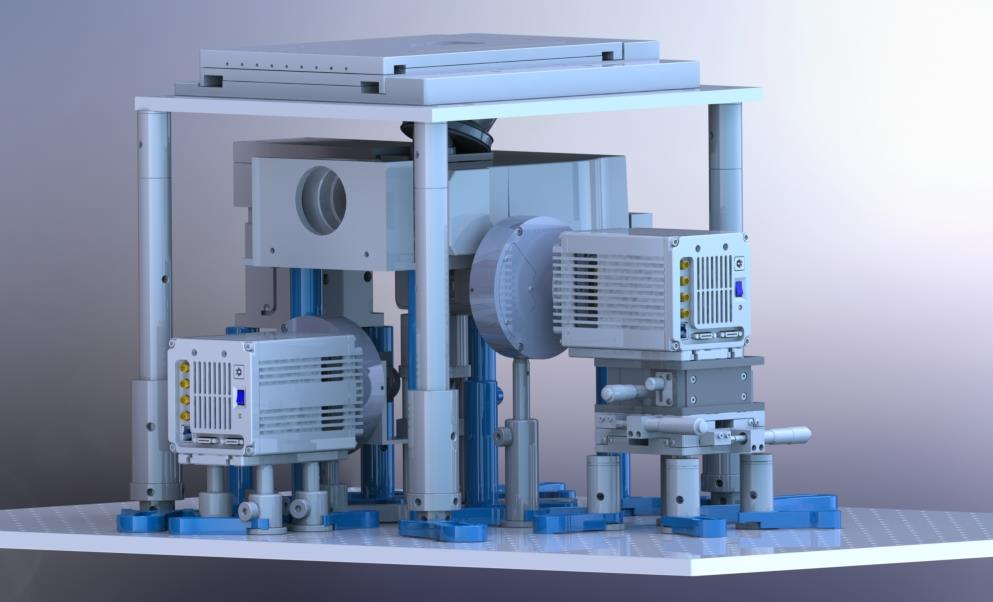
\includegraphics[width=0.78\linewidth]{../figures/2/FRETScope示意图.jpg}
  \caption{FRETScope硬件外观示意图}
  \label{fig:fretscope2硬件示意图}
\end{figure}
\begin{figure}[htbp]
  \centering
  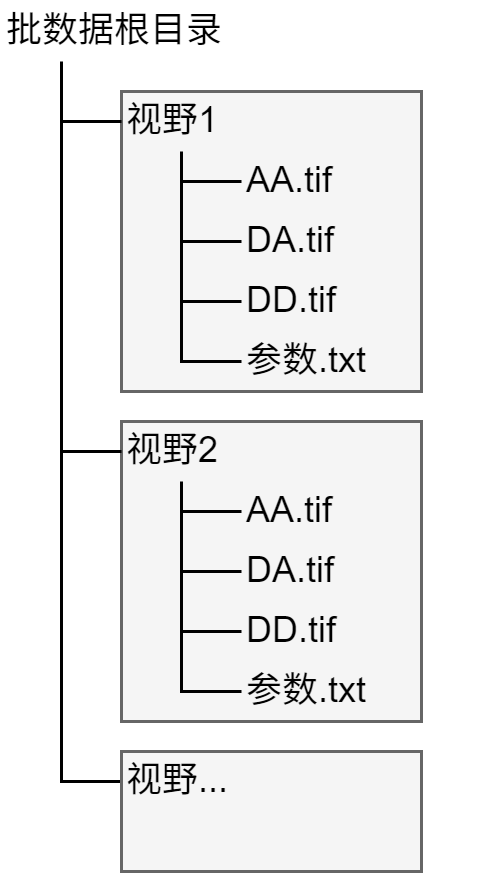
\includegraphics[height=0.55\linewidth]{../figures/2/FRETScope数据格式.drawio.png}
  \caption{FRETScope数据文件结构}
  \label{fig:fretscope_data_struct}
\end{figure}

\subsection{FRET双杂交分析数据处理流程}
\begin{figure}[hbtp]
  \centering
  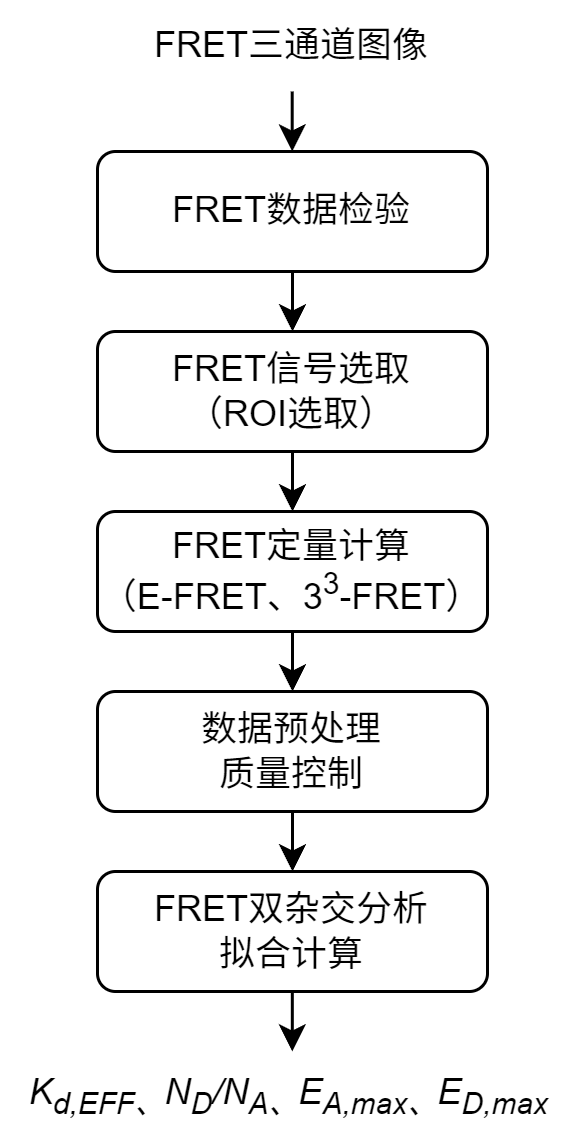
\includegraphics[width=0.4\linewidth]{../figures/2/双杂交数据处理流程.drawio.png}
  \caption{FRET双杂交分析数据处理流程}
  \label{fig:tha_data_process}
\end{figure}
使用FRETScope对制备好的样本进行图像采集得到若干视野的FRET三通道图像后,通过FRET双杂交分析方法定量计算细胞中的生物大分子结合作用的FRET饱和效率、化学计量比、相对亲和力等信息。
FRET双杂交分析的数据处理需要如下步骤:
首先需要对FRET数据进行数据完整性校验,确保每个视野下存在完整的三通道图像和文件完整可读,然后对每个视野进行荧光信号提取,通过在图像上绘制ROI并计算其灰度均值作为FRET分析计算重要的荧光信号;
根据E-FRET和$3^3$-FRET方法将上述荧光信号代入对应的计算公式 \ref{eq:ed}、\ref{eq:rc} 和 \ref{eq:ea} 求取$E_A$、$E_D$、$R_C$等FRET数据;
对这些数据进一步依据物理含义或者数据分析进行异常值去除等数据预处理;
最后是通过优化算法拟合Langmiur模型或者线性模型计算相关的参数。
具体流程如图 \ref{fig:tha_data_process} 所示。

\subsection{模块划分和界面设计}
结合 FRET 双杂交分析的数据处理流程与功能逻辑,Fretha 软件主要划分为以下核心模块:
\begin{enumerate}
  \item {成像参数设置模块:}
  负责设置 FRET 成像过程中的成像参数,在不同实验数据处理前,需要更新对应地参数。
  该模块允许用户输入和保存成像参数,如曝光时间、串扰系数和校正因子等,并提供参数校验功能,确保参数在合理范围内,避免因参数设置错误导致数据分析处理异常。
  此外,该模块还支持将参数持久化到本地,以供多次处理数据时使用。
  \item {数据检验模块:}
  对输入数据进行命名规范和完整性等合法性检验,防止用户输入异常数据导致软件错误。
  该模块按照FRETScope系统的数据结构特征,检查每个子视野的三通道图像文件是否完整,并对文件格式和内容进行验证,确保数据的可靠性。
  \item {FRET 图像处理模块:}
  支持手动图像处理和 ROI 选取,满足用户对数据的精细化处理需求。
  手动选取感兴趣区域ROI是一个基础且关键的操作,它能帮助分析人员聚焦于细胞中荧光质量较高的区域,进行更精确的数据处理与分析。
  用户可以选择启用图像增强功能,比如归一化增强视图、生成FRET效率伪彩图等,从而提高ROI标注时的参考信息。
  该模块还提供ROI状态栏,实时计算ROI的荧光信号、视野背景、敏化发射荧光和E-FRET计算结果等,可以为ROI的质量判定提供参考。
  \item {数据管理模块:}
  数据处理模块用于增删数据、筛选数据、导入导出、开始计算等功能,还可以数据项反向定位追踪FRET图像中的ROI详情,以便检查数据和再处理。
  该模块作为FRET图像处理模块和结果可视化模块的桥梁,负责数据的统一管理和高效传递。
  \item {结果可视化模块:}
  将分析结果以直观的图表形式展示,并提供数据保存功能,方便用户进一步分析和应用。
  用户可以根据需要选择L-FRET或者DC-FRET方法的对应视图,以切换FRET双杂交分析方法。
  该模块通过在同一坐标系下绘制趋势线图和散点图,用户可以更直观地评估FRET双杂交分析计算拟合程度等。
  结果可视化模块还可以将分析结果保存为图片或数据文件,方便用户进行后续数据处理和报告撰写。
  
\end{enumerate}

在界面设计上,根据软件使用需求和模块功能,主要分为:开始页、参数设置页、数据处理页、结果页。
在软件开始页提供了跳转参数设置页或数据处理页的按钮,如图 \ref{fig:开始页界面} 所示;
\begin{figure}[hbtp]
  \centering
  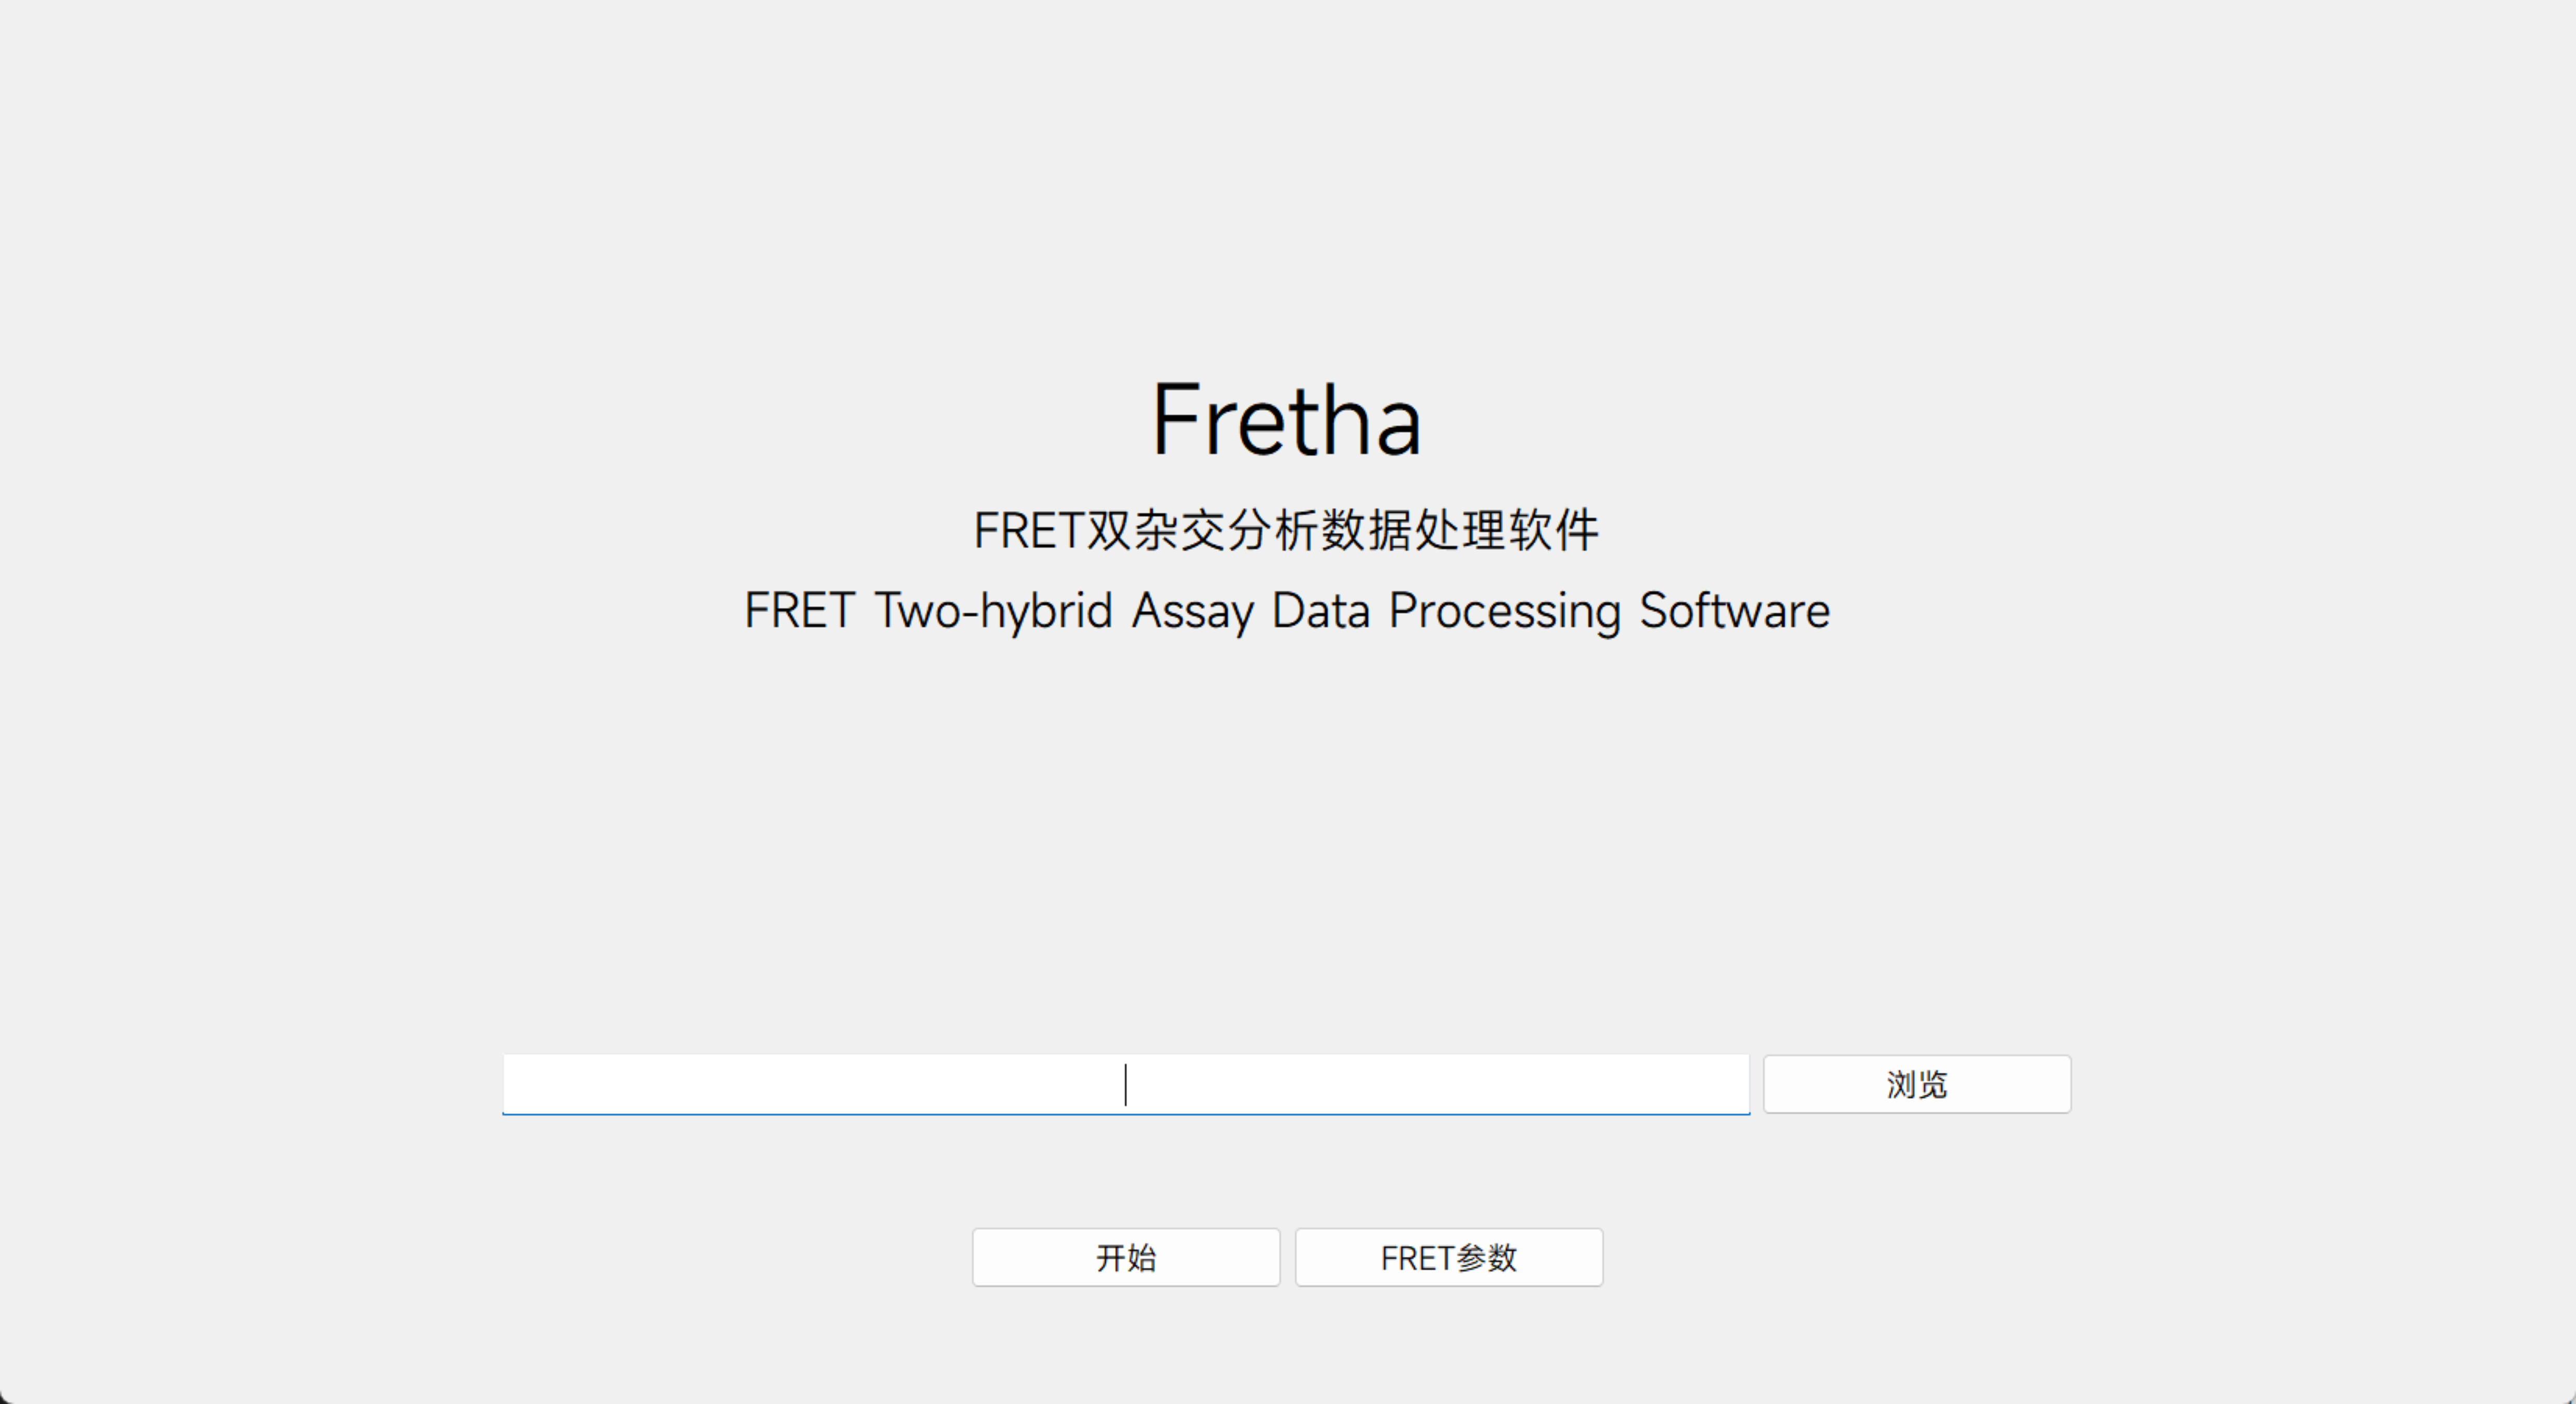
\includegraphics[width=0.9\linewidth]{../figures/2/Fretha界面-开始界面.drawio.png}
  \caption{Fretha开始页界面}
  \label{fig:开始页界面}
\end{figure}
参数设置页面包括成像参数设置模块,其界面如图 \ref{fig:参数设置页界面} 所示;
\begin{figure}[hbtp]
  \centering
  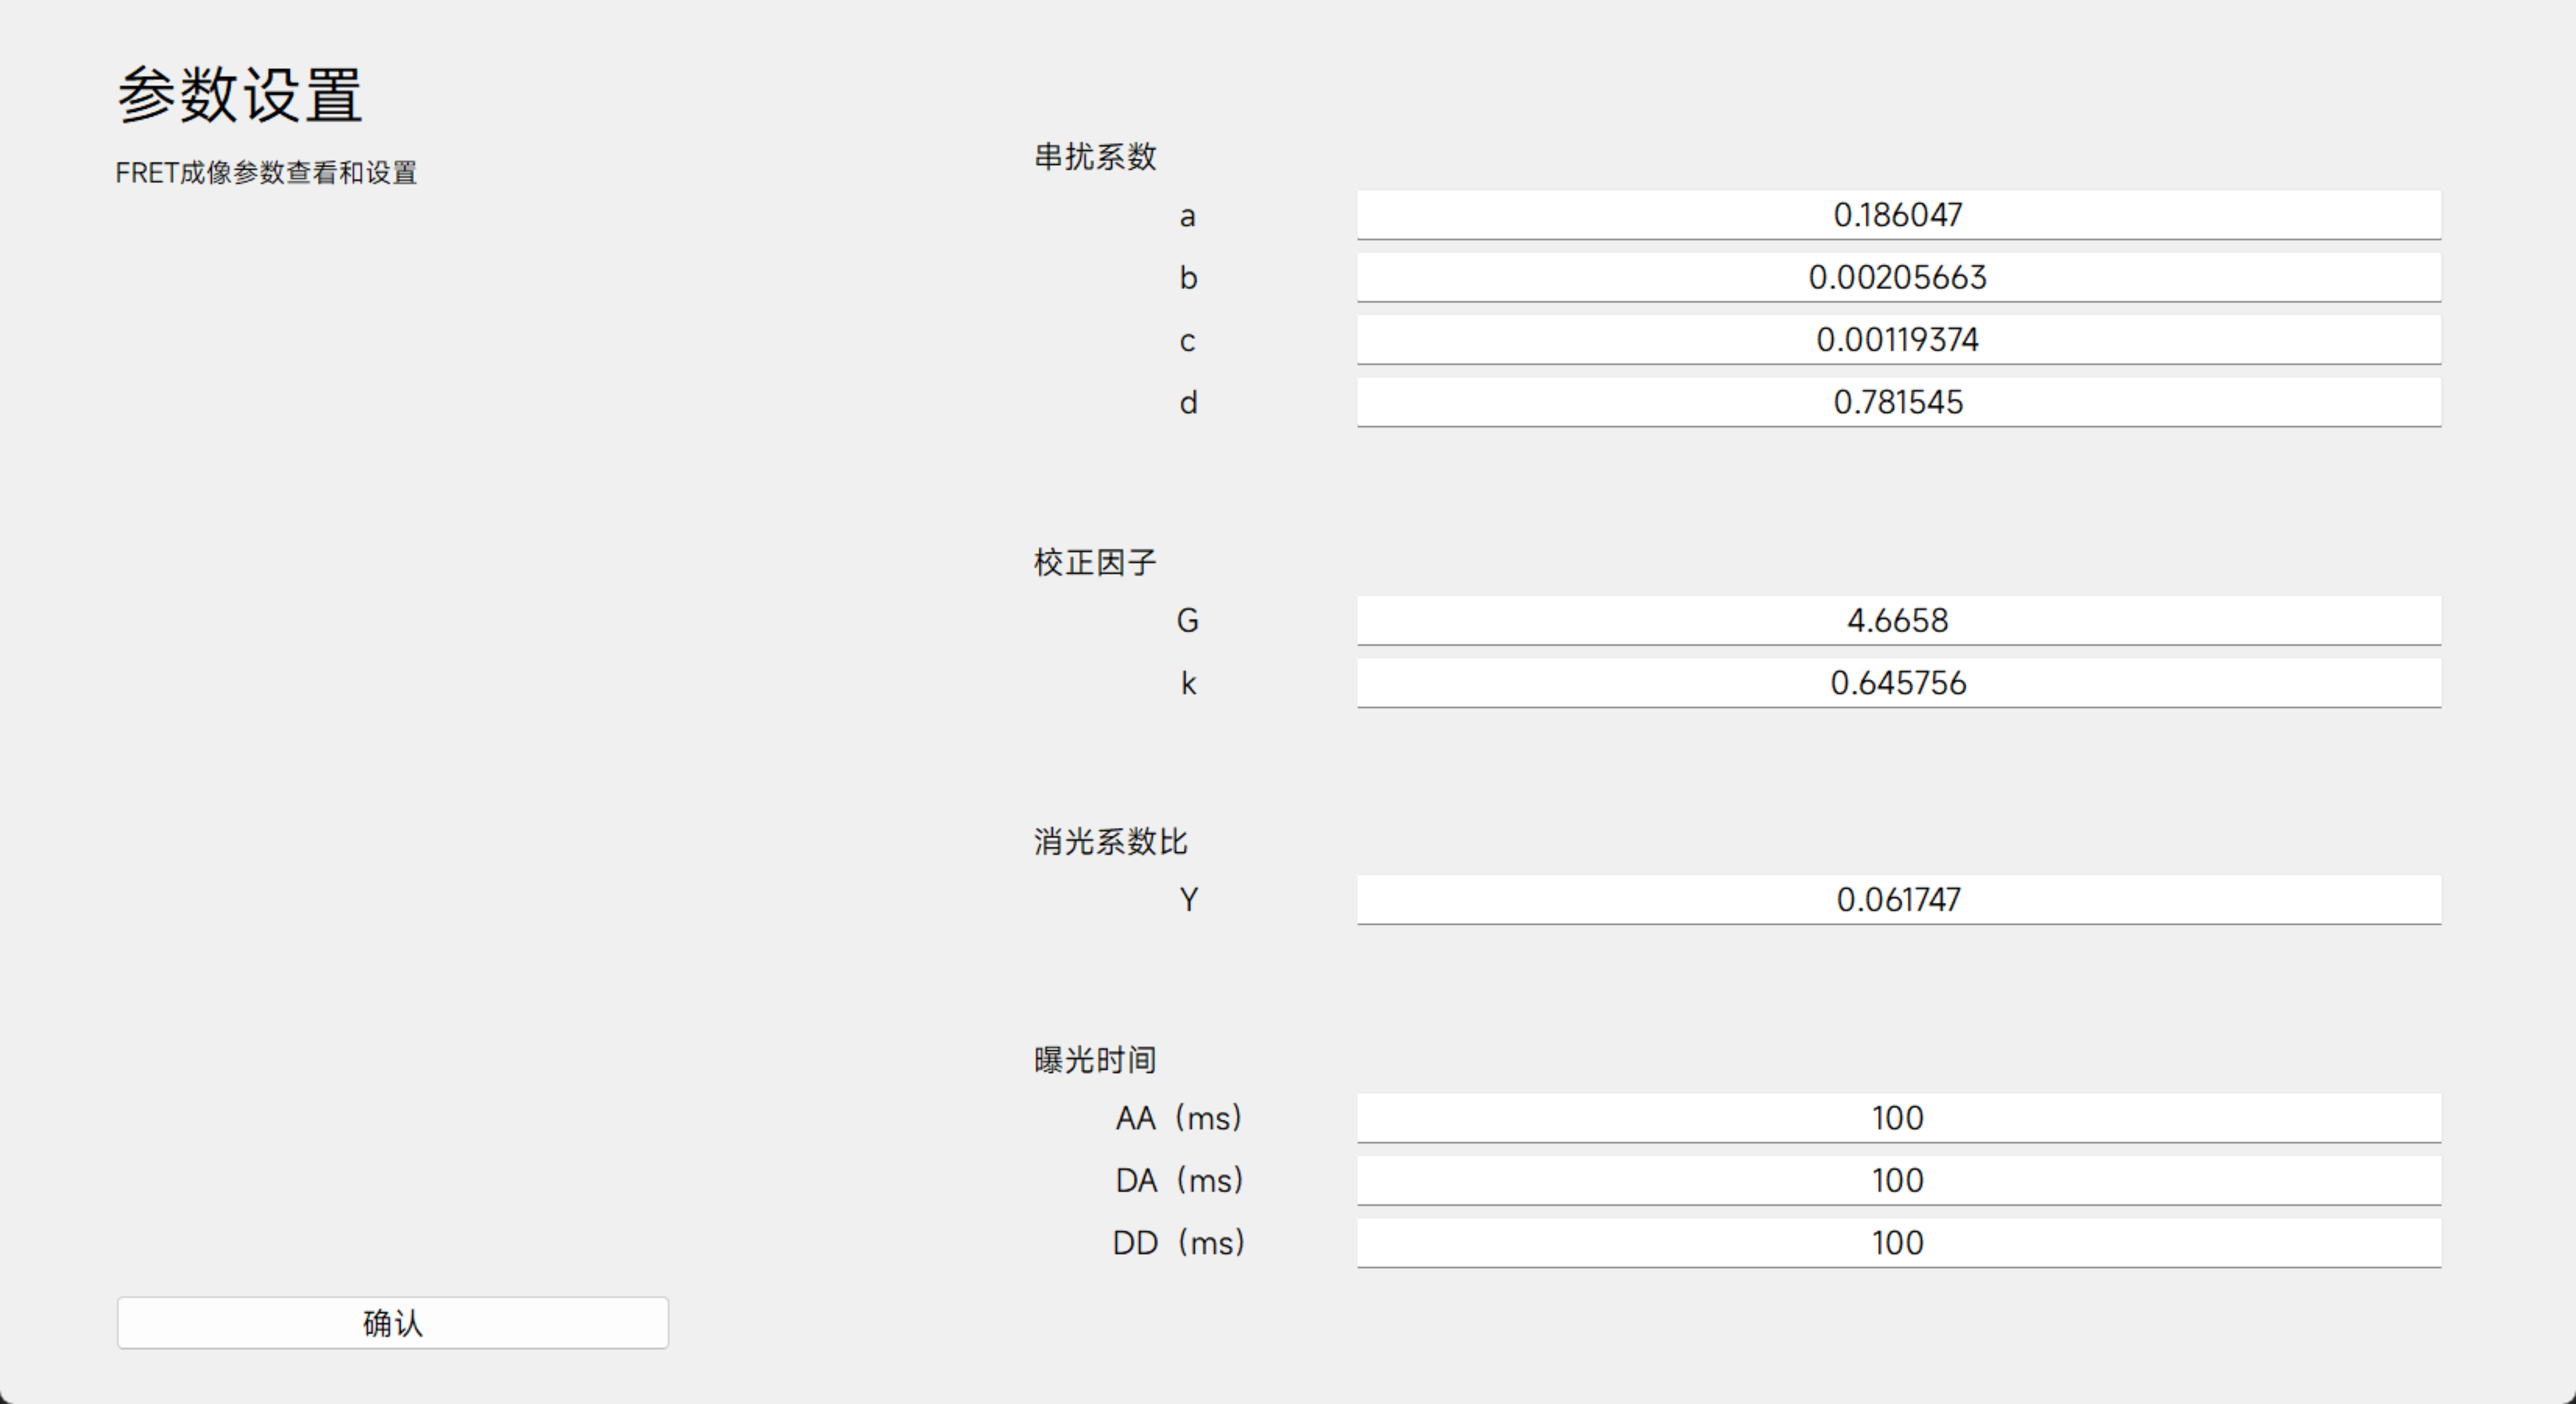
\includegraphics[width=0.9\linewidth]{../figures/2/Fretha界面-参数设置.drawio.png}
  \caption{Fretha参数设置页界面}
  \label{fig:参数设置页界面}
\end{figure}
数据处理页包括数据检验模块的检验结果、FRET图像处理模块、数据管理模块,其界面和模块划分如图 \ref {fig:界面模块分布图} 所示;
\begin{figure}[hbtp]
  \centering
  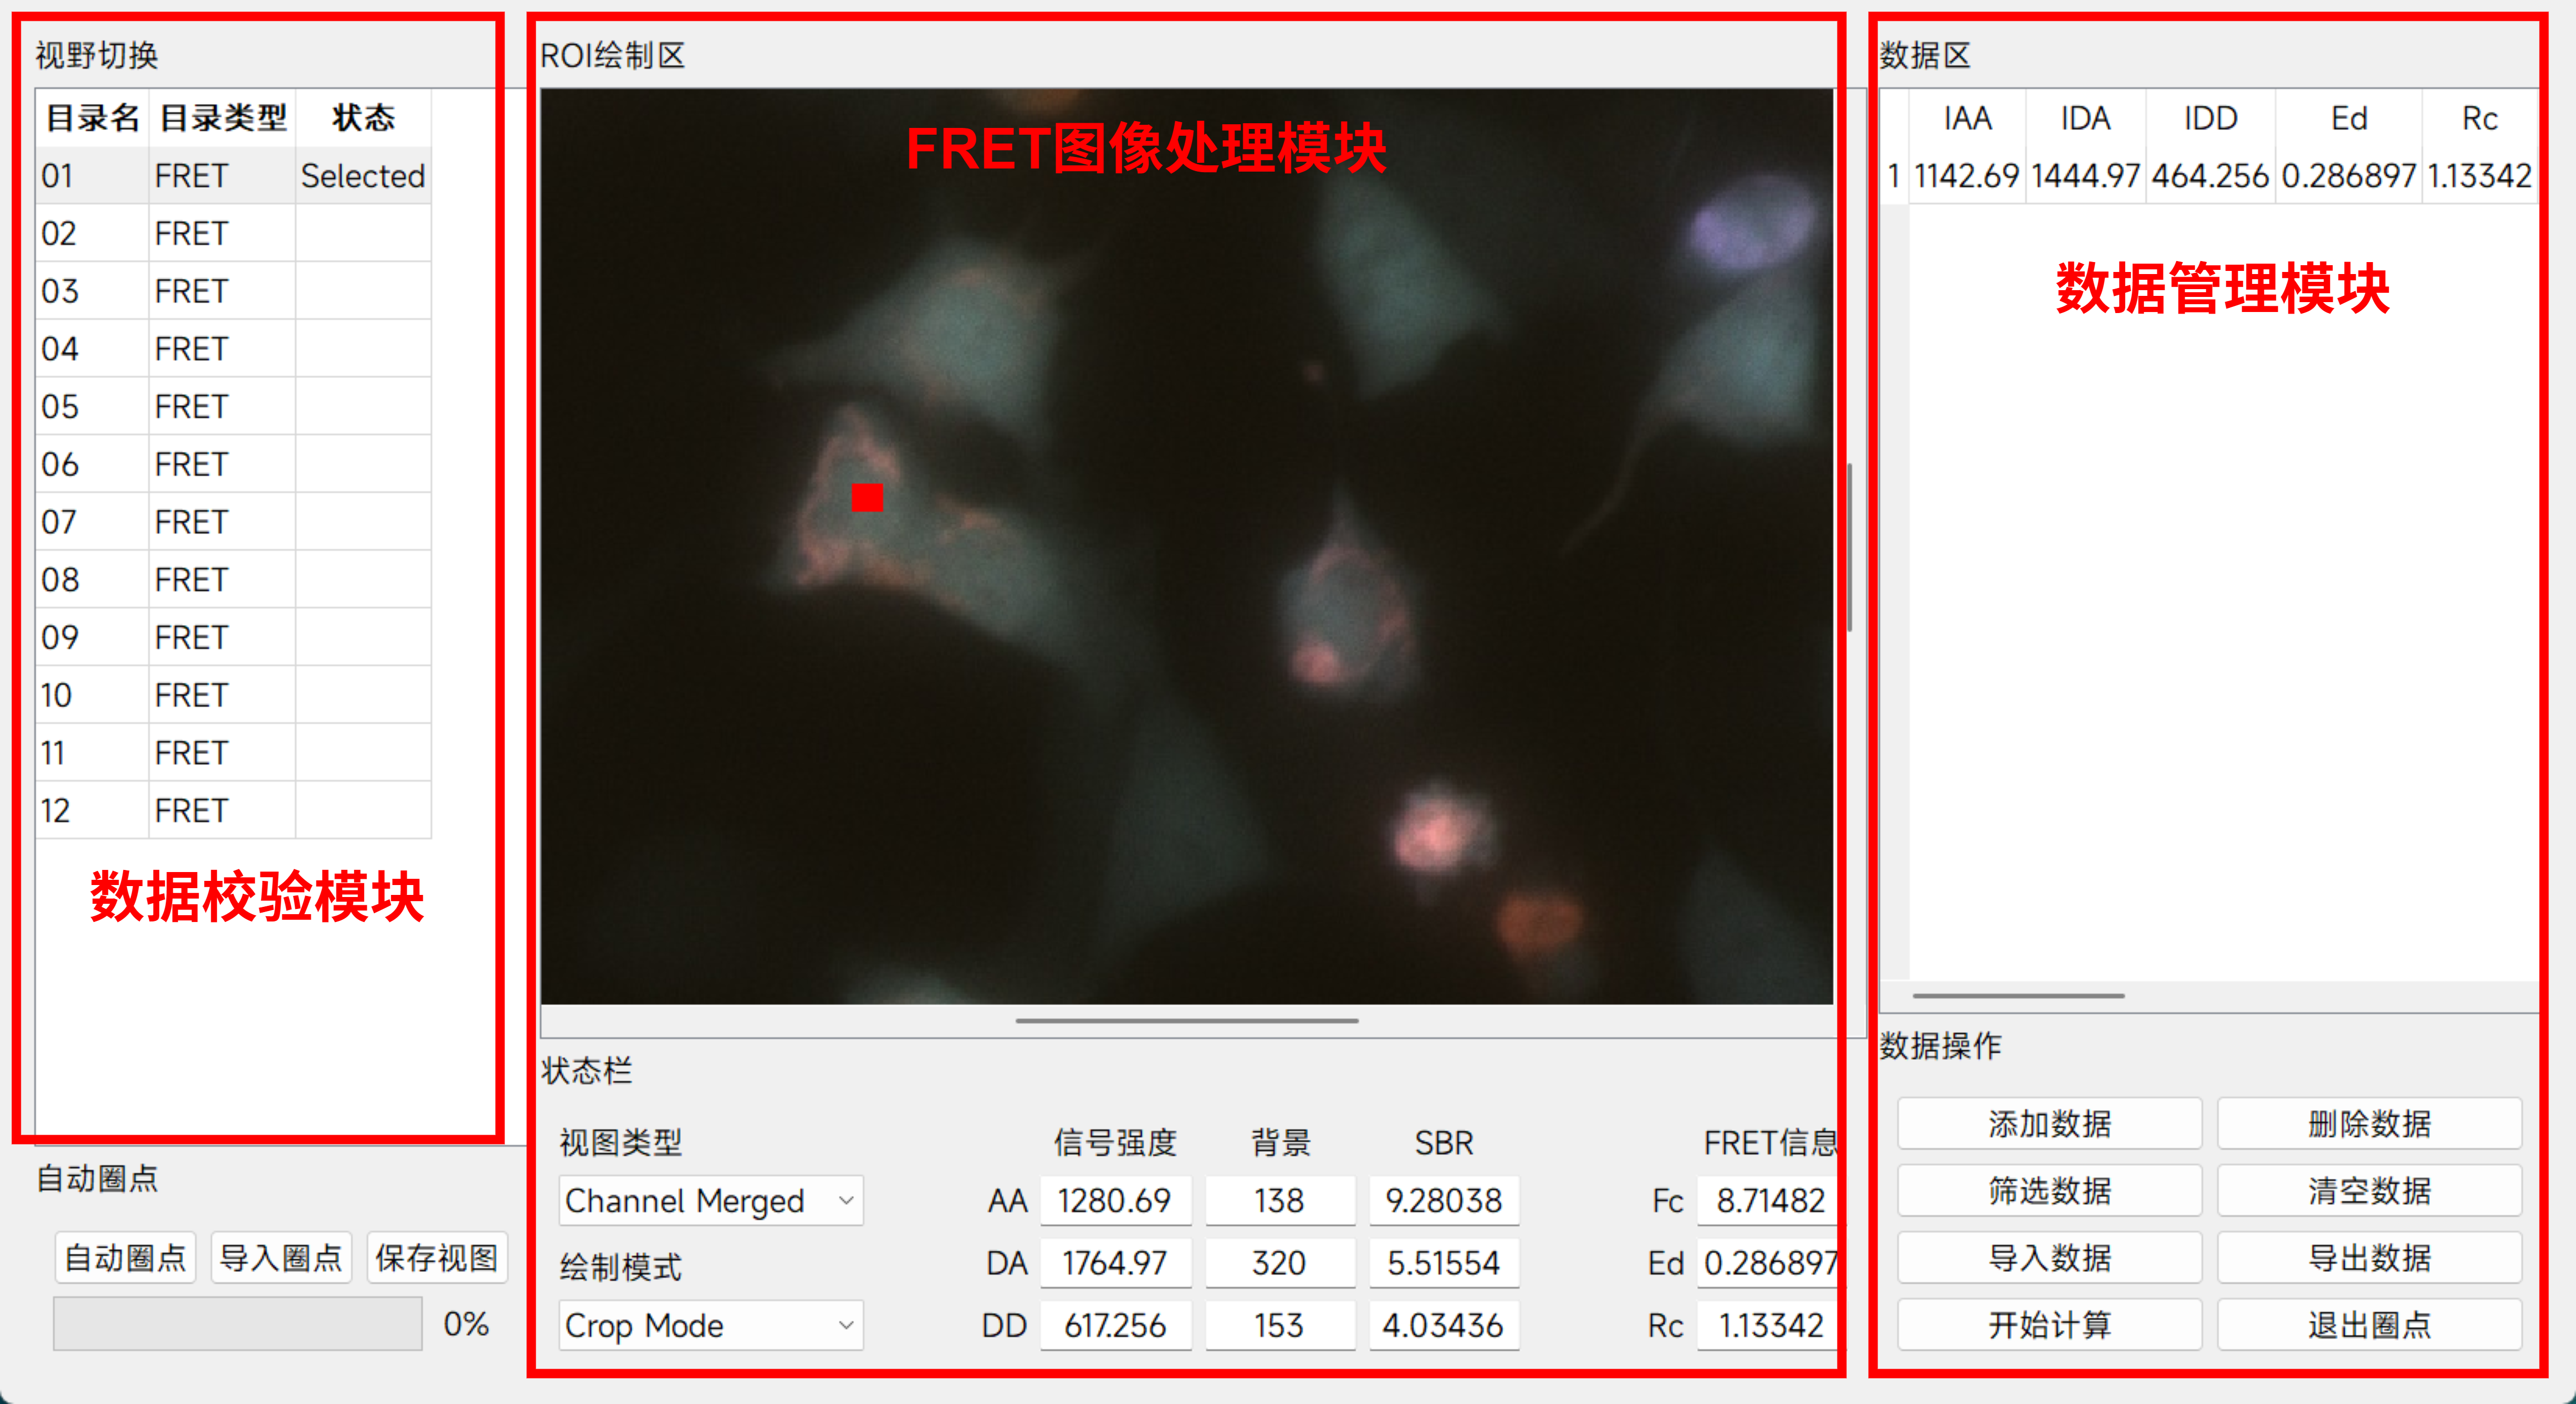
\includegraphics[width=0.9\linewidth]{../figures/2/Fretha界面-数据处理.drawio.png}
  \caption{Fretha数据处理页界面及模块划分}
  \label{fig:界面模块分布图}
\end{figure}
结果页展示结果可视化模块中FRET双杂交数据处理的图像视图结果,提供了结果可视化、视图切换和结果保存等界面,如图 \ref{fig:Fretha结果可视化模块界面} 所示。
\begin{figure}[hbtp]
  \centering
  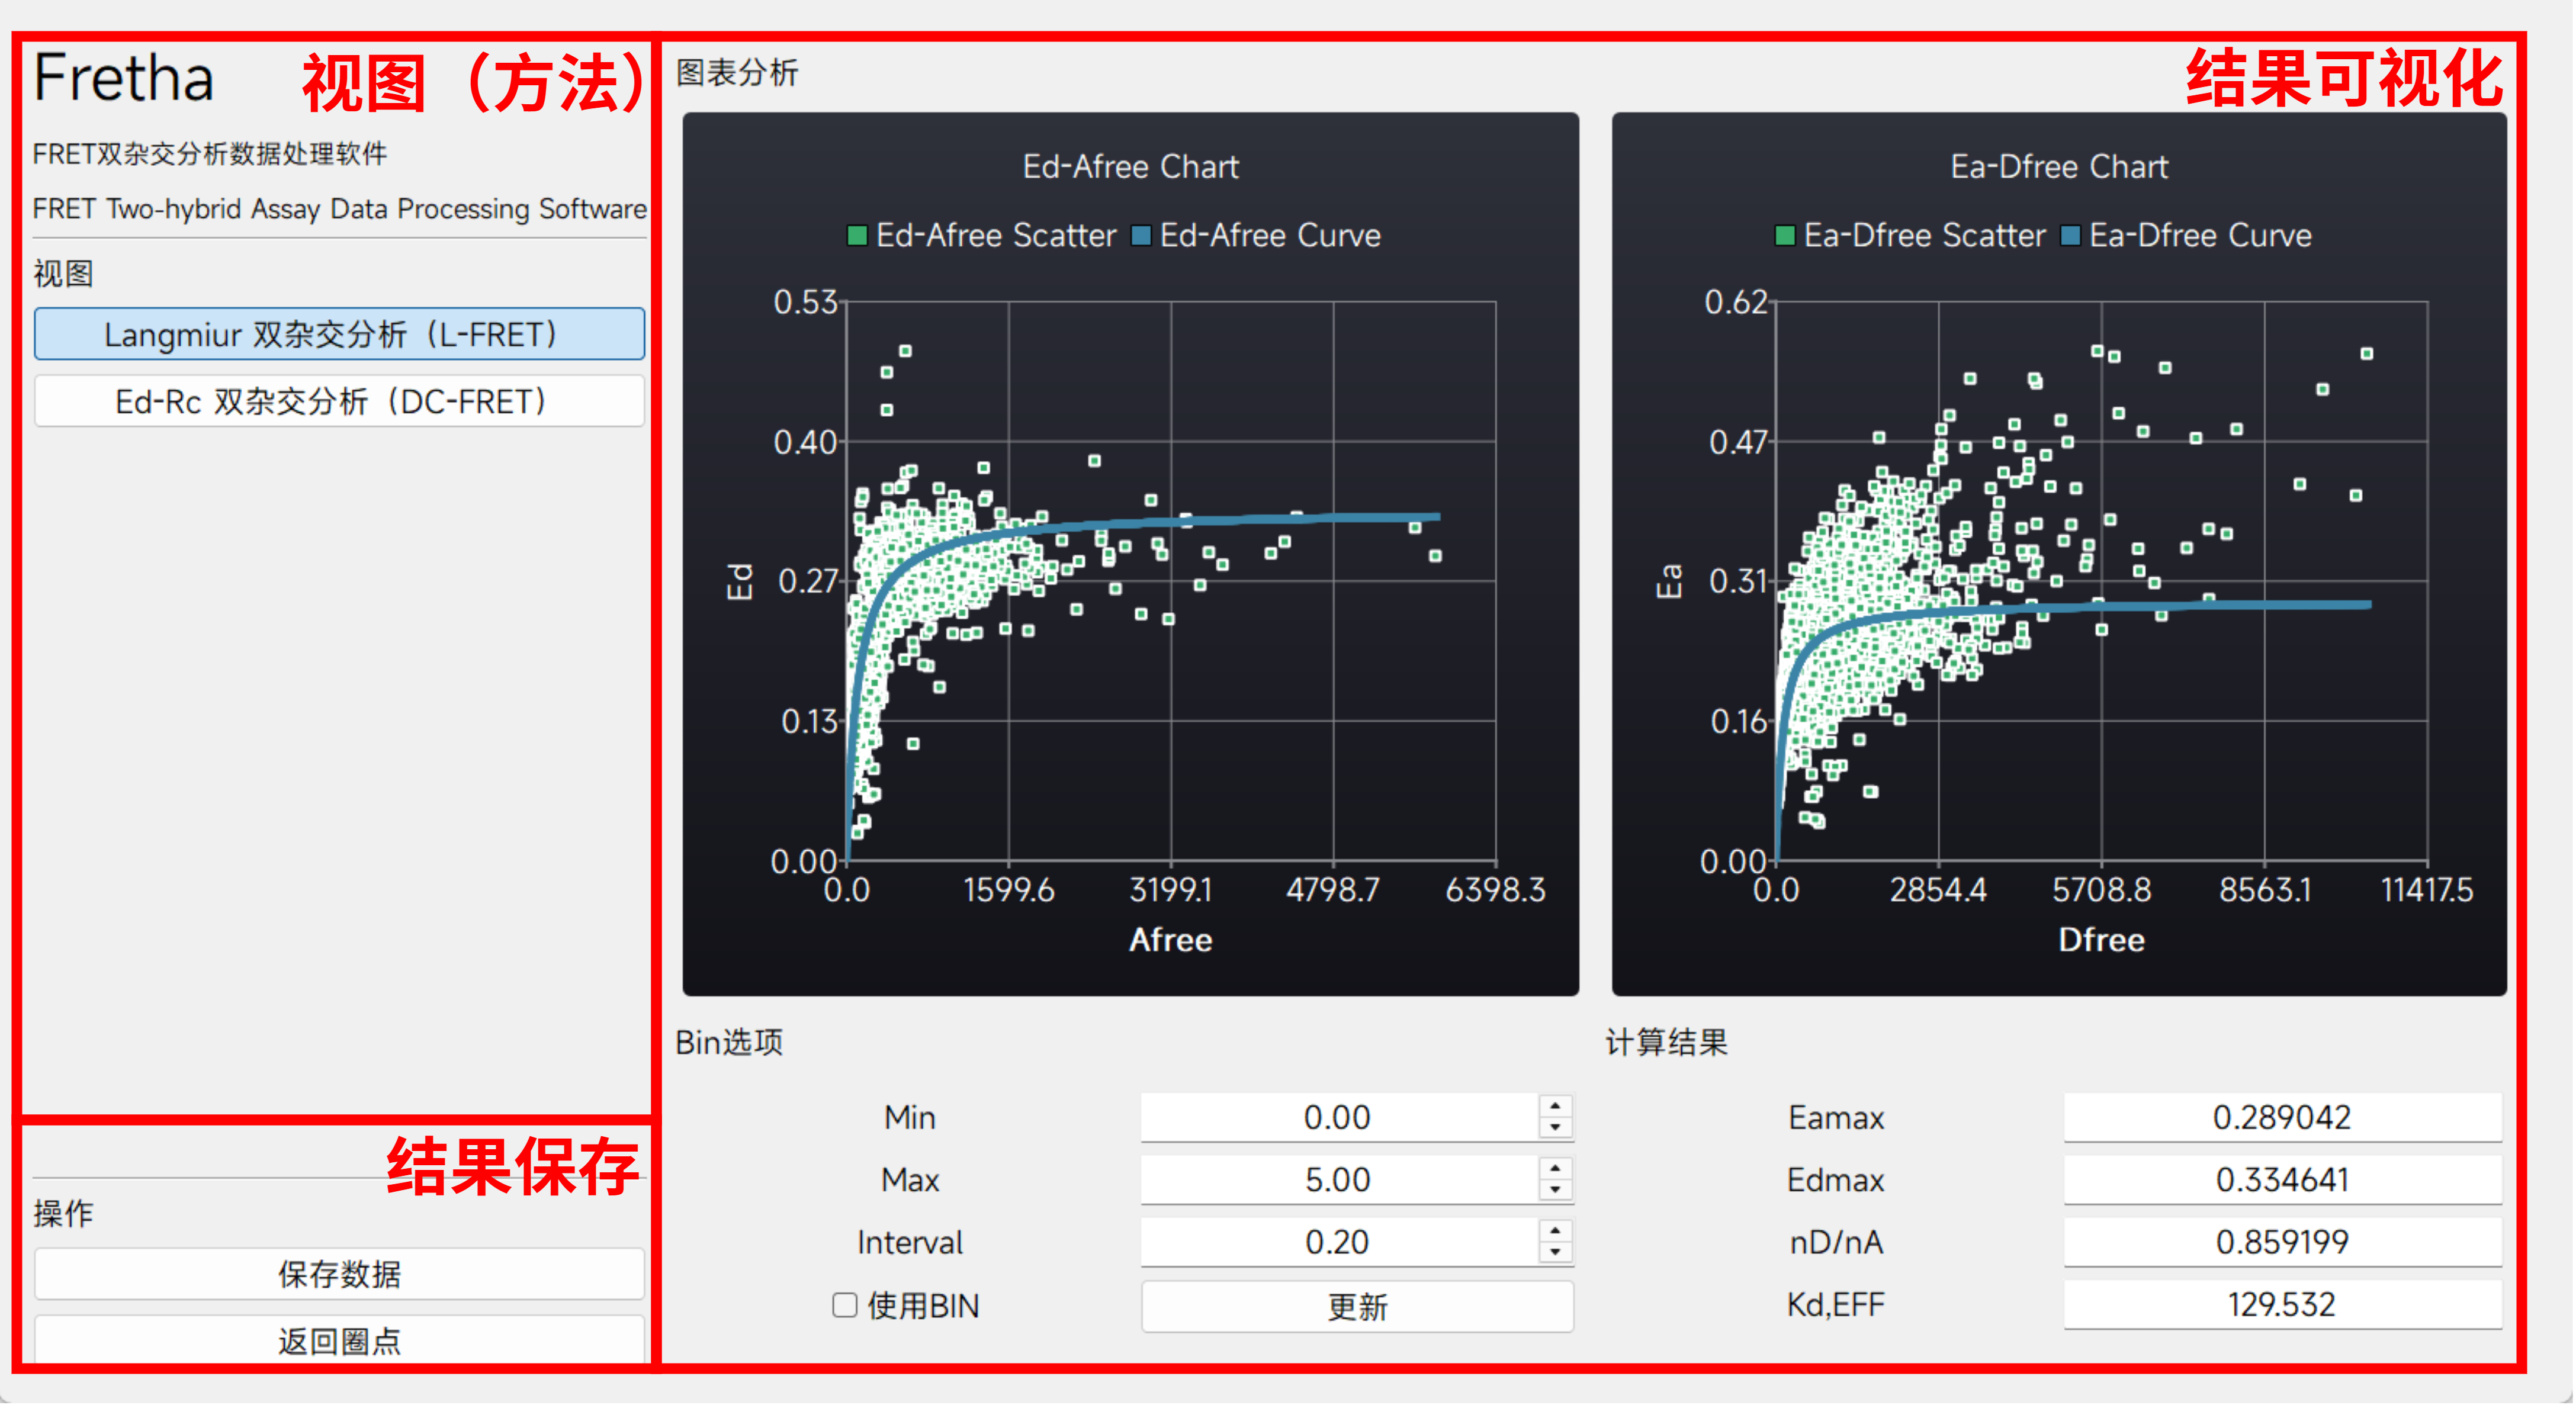
\includegraphics[width=0.9\linewidth]{../figures/2/Fretha界面-结果展示.drawio.png}
  \caption{Fretha结果可视化模块界面}
  \label{fig:Fretha结果可视化模块界面}
\end{figure}

\subsection{软件总体框架}

Fretha架构采用分层设计,由顶层向下依次分别为:表现层、业务层、数据访问层和数据层,如图 \ref{fig:fretha_arch} 所示。
\begin{figure}[hbtp]
    \centering
    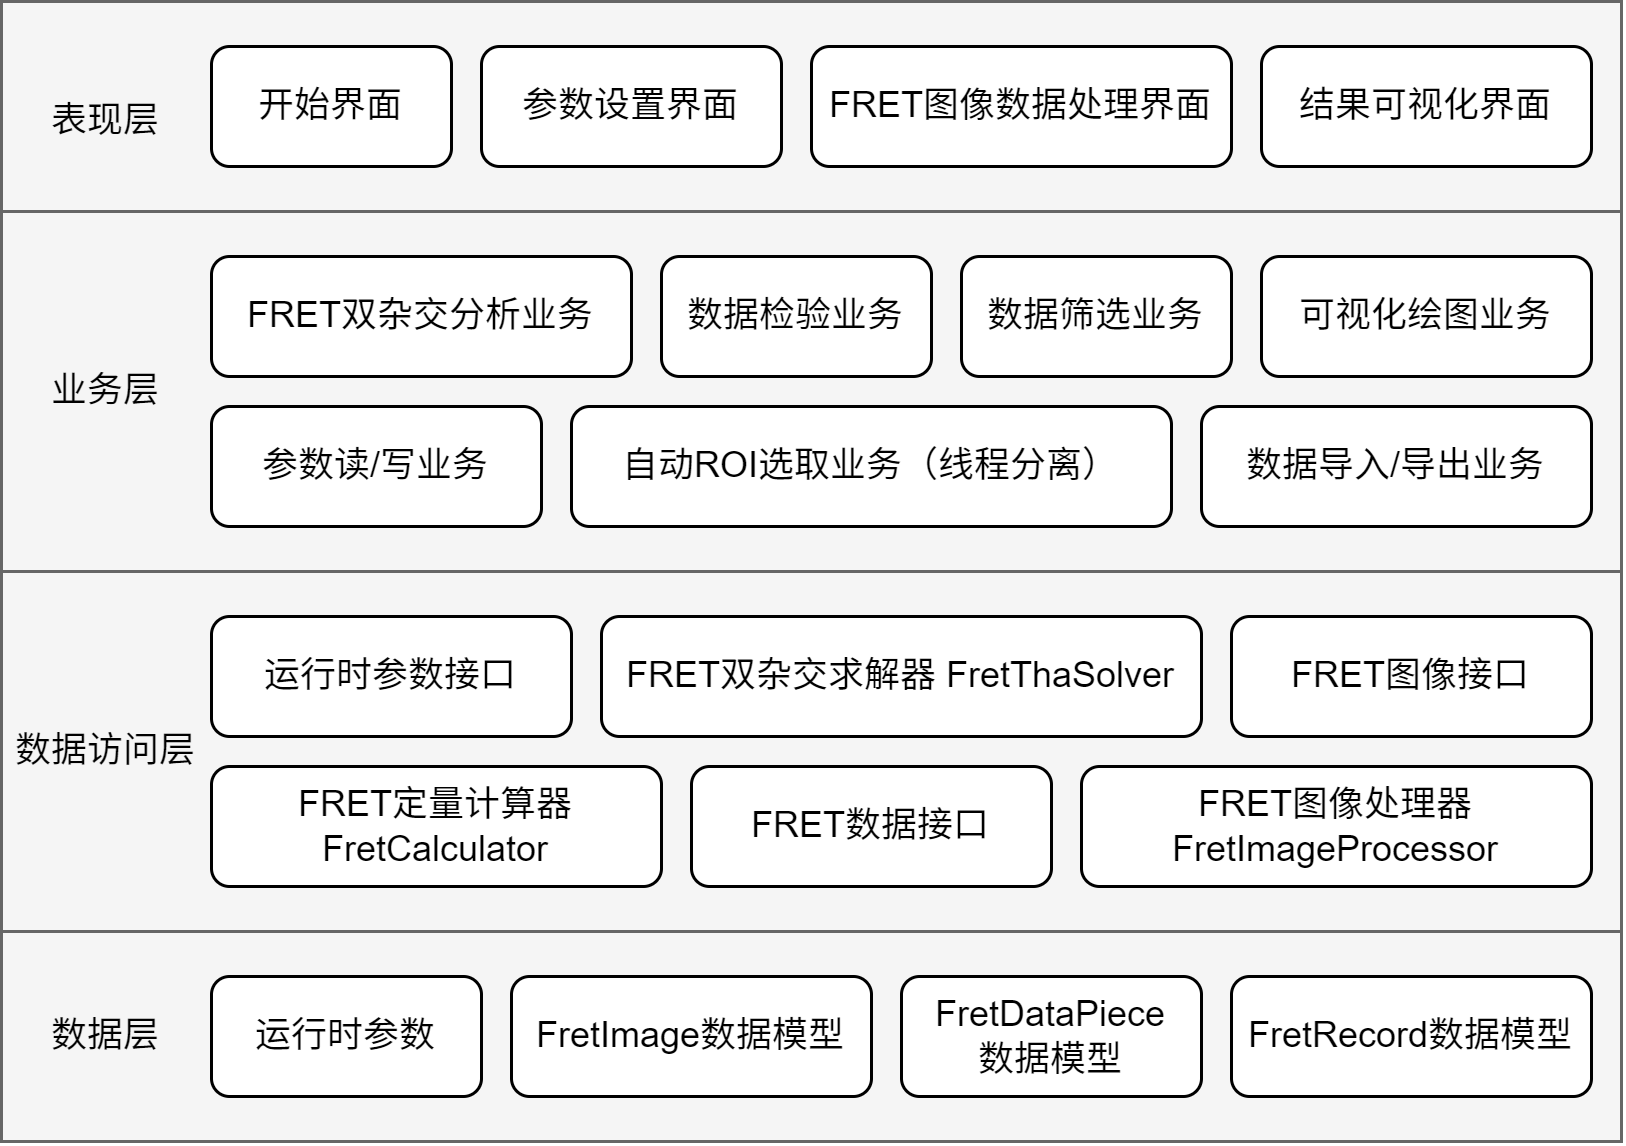
\includegraphics[width=0.9\linewidth]{../figures/2/Fretha总体架构图.drawio.png}
    \caption{Fretha软件总体架构}
    \label{fig:fretha_arch}
\end{figure}

表现层(Presentation Layer)处于整个架构的最上层,是用户与系统进行交互的主要界面。
表现层通过QtCreator静态构建结合QML动态创建,负责接收用户输入的操作和数据,并以直观、友好的方式展示系统的处理结果。
表现层主要包括开始界面、参数设置界面、FRET图像处理界面、结果可视化界面等。
Fretha通过表现层的设计约束了用户的操作流程和操作规范,规范化了FRET双杂交分析数据处理的过程。

业务层(Business Logic Layer)是整个架构的核心逻辑处理部分,承担着具体模块功能和其对应的业务逻辑的实现。
业务层接收来自表现层的请求,根据预设的业务逻辑对数据进行处理和转换。
Fretha的业务层封装了包括参数读/写业务、数据检验业务、自动ROI选取业务、数据导入/导出业务、FRET双杂交分析业务、可视化绘图业务等。

数据访问层(Data Access Layer)实现对数据的访问和操作,将业务层与数据层进行隔离。
业务层通过调用数据访问层提供的接口来获取和操作数据,无需关心数据的具体存储方式和位置。
通过设置数据访问层,能够使得在复杂的业务处理时避免对数据的直接操作和影响,从而提高了数据存储的安全性。
Fretha的数据访问层包括FRET图像数据访问、FRET数值数据访问和FRET双杂交数据访问的接口。
特别地,在数据访问层还包括FRET定量计算器和FRET图像处理器、FRET双杂交求解器等,它们除了可以作为数据访问层的接口,还可以完成FRET计算分析作为业务层的业务逻辑处理单元,这样的设计减少了业务层设计的复杂度,提高了系统的可维护性和可扩展性。

最后是数据层(Data Layer),作为架构的最底层,数据层负责存储系统的所有数据。
Fretha数据层包括系统静态数据、FretImage模型、FretDataPiece模型和FretRecord模型。
系统静态数据是在软件运行时的环境参数,只需要在指定步骤运行前提前设置好即可,如成像参数、文件目录等。
FretDataPiece、FretImage和FretRecord用来存储和计算各种动态数据。
在FRET双杂交分析数据处理中,一个视野下的FRET三通道图像存储于FretImage中,从中可以提取并计算出若干条FRET数据FretDataPiece,由若干视野作为一个批次只能解析出一条FRET双杂交分析结果FretRecord。
因此,在设计上三种数据实体类型存在关联关系,FretDataPiece和FretImage之间存在一对多关系,FretImage和FretDataPiece之间存在一对多的关系,如图 \ref{fig:fretha_data_relations} 所示。
\begin{figure}[hbtp]
    \centering
    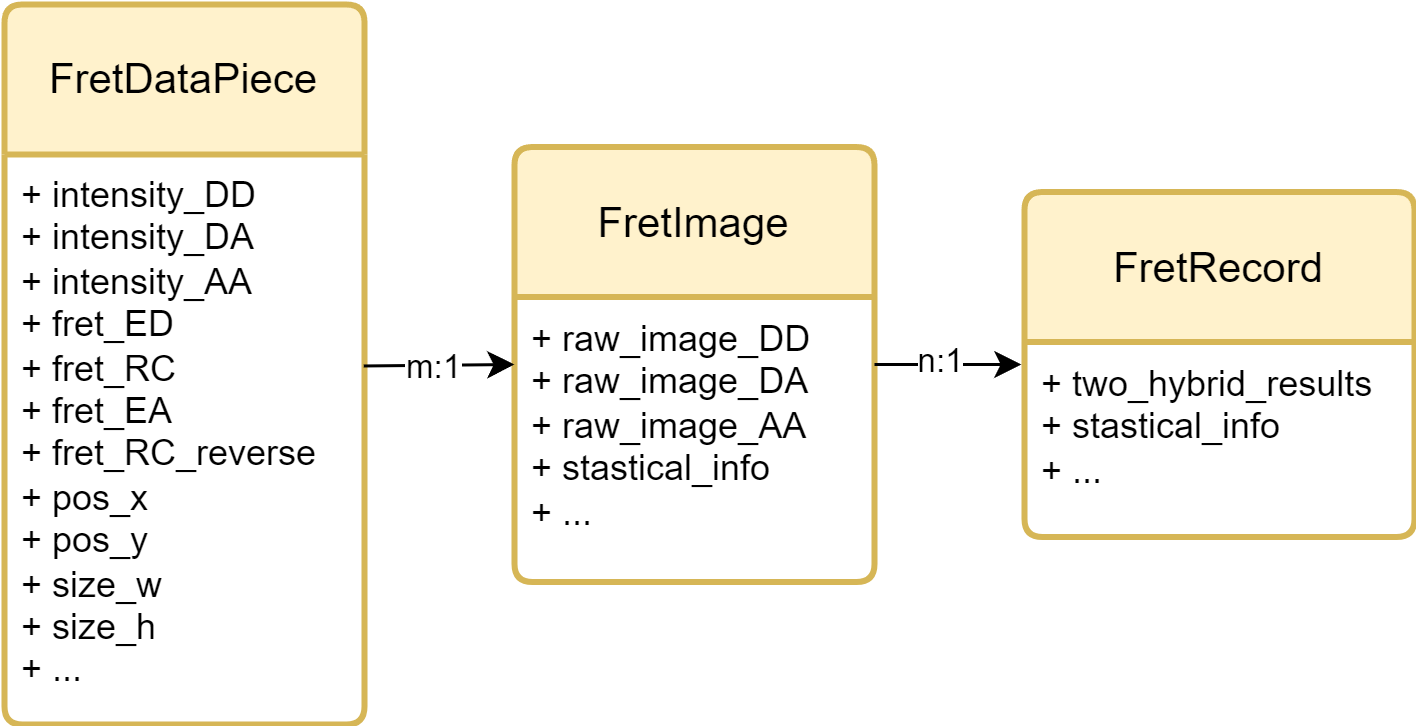
\includegraphics[width=1\linewidth]{../figures/2/Fretha数据模型.drawio.png}
    \caption{Fretha数据层实体关联关系图}
    \label{fig:fretha_data_relations}
\end{figure}

\subsection{开发技术选型}
Qt是目前最流行的跨平台应用程序和 UI 开发框架之一,广泛应用于桌面、嵌入式和移动设备等领域。
Qt提供了可靠的C++类库,提供了良好的跨桌面和嵌入式操作系统的移植性,包括:
(1)图形用户界面(Graphics User Interface, GUI):提供了按钮、文本框、对话框等完整的控件,以及支持控件的自定义;
(2)多线程:方便开发者管理线程,数据和对象,且基于信号和槽机制实现了线程间的安全通信;
(3)OpenGL支持:可以在构建支持硬件加速的高性能可视化应用程序,提高对系统资源的利用。
Qt 5.15.2是Qt官方发布的长期支持(Long Term Support, LTS)版本,本文选择Qt 5.15.2作为Fretha的开发框架。

OpenCV(Open source computer vision library)是一个跨平台开源计算机视觉库。
它轻量级且高效,C++版本由一系列C函数和C++类构成,同时提供了Python、MATLAB等语言的接口。
OpenCV 提供了大量的计算机视觉算法和图像处理工具,广泛应用于图像和视频的处理、分析以及机器学习领域\upcite{singh2022face, adusumalli2021face}。
主要提供的功能库包括:
(1)图像处理:提供了经典的图像滤波、边缘检测、颜色空间转换、形态学操作、特征提取等算法;
(2)视频分析: 视频捕捉、运动分析、物体检测与追踪等;
(3)机器学习与人工智能: OpenCV 正在不断完善对深度学习和人工智能技术的支持,如人脸识别、目标检测、图像分类等方法。
OpenCV 的很多算法都经过高度优化,支持硬件级别的加速,因此在处理复杂计算功能时具备高性能。
鉴于这些优势,OpenCV 被选为 Fretha 图像处理模块的核心技术方案。

Dlib提供了和机器学习、数值计算、图模型算法、图像处理等领域相关的一系列功能,广泛应用于工业界和学术界,包括机器人,嵌入式设备等高性能计算环境。
L-FRET方法的参数拟合计算是一个非线性约束优化问题,Dlib能够高效地完成求解计算。
Dlib整合了梯度优化算法与自适应学习率策略,在保证收敛速度的同时减少了陷入局部最优的风险。
算法实现上,Dlib 结合了牛顿法和类牛顿方法,这种组合既保留了牛顿法的高精度特性,又通过拟牛顿近似提升了计算效率。
在约束优化问题上,还支持通过内点法解决资源分配中的约束问题。
综合Dlib的上述优点,本文选择Dlib作为Fretha的FRET双杂交求解器的计算支持工具。

\section{FRET算法和后台接口}

\subsection{FRET定量计算器}
FRET定量计算器(FretCalculator)用于处理E-FRET和$3^3$-FRET定量计算,用于将输入的三通道荧光信号转换为定量FRET信息如$E_A$、$E_D$和$R_C$等。
如图 \ref{fig:fretha_calculator} 所示,FRET定量计算器在实例化后需要经过成像参数设置、加载荧光数据、数据校正、数据计算和结果获取等计算步骤,每个步骤需要按照顺序执行,并且在执行时记录运行状态,在获取结果数据之前进行检查来保证数据安全。
\begin{figure}[hbtp]
  \centering
  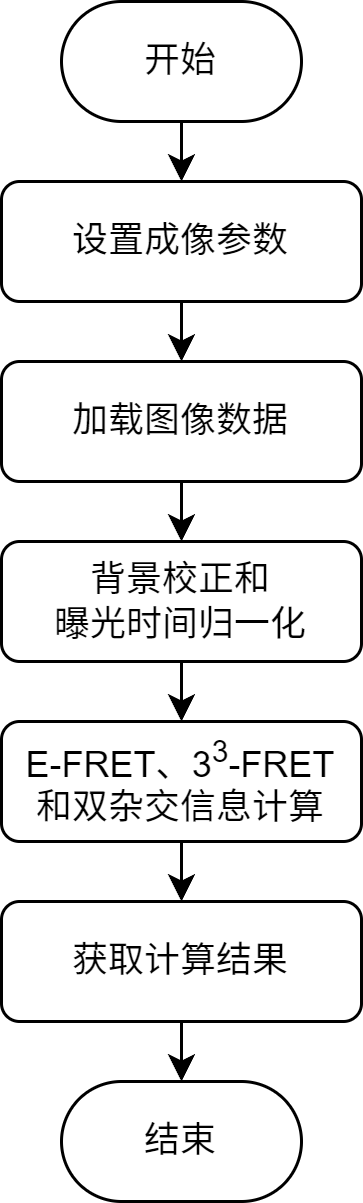
\includegraphics[width=0.25\linewidth]{../figures/2/FRET计算器计算步骤.drawio.png}
  \caption{FretCalculator计算步骤}
  \label{fig:fretha_calculator}
\end{figure}

参数设置中,FretCalculator读取系统静态数据中的成像参数,用于在计算中使用。
通过接口函数加载$I_{DD}$、$I_{DA}$、$I_{AA}$数据到FretCalculator实例的数据成员中,然后
数据校正中,FretCalculator对FRET图像数据进行背景值估计和荧光强度校正,并按照曝光时间进行归一化。
校正后的数据根据E-FRET和$3^3$-FRET方法对荧光强度进行计算,得到FRET定量计算结果$E_D$和$R_C$等。
最后FretCalculator可以返回指定计算结果给调用者。

特别地,除了支持E-FRET和$3^3$-FRET定量计算外,FretCalculator还可以计算L-FRET方法中需要的供体分子数估值$D_{est}$和受体分子数估值$A_{est}$。计算公式如下:
\begin{align}
  M_A/M_D &= G \cdot \frac{\varepsilon_D/\varepsilon_A}{d}, \\
  D_{est} &= d \cdot I_{DD} / (1 - E_D), \\ 
  A_{est} &= \frac{a \cdot (I_{AA} - c\cdot I_{DD})} {M_A/M_D},
\end{align}
其中,$M_A/M_D$是单个供体分子的亮度和单个受体分子亮度之比。

\subsection{FRET图像处理器}
FRET图像处理器(FretImageProcesser)封装了对FRET图像进行定量FRET计算的相关功能,其计算步骤和FretCalculator类似,如图 \ref{fig:fretha_calculator} 所示。
FretImageProcesser接收和返回的数据类型是OpenCV的Mat数据结构,可以方便地存储和处理图像数据和逐像素的FRET图像数据。
FRET图像分析时需要对每个像素点的荧光强度进行计算,对图像数据进行遍历处理。

此外,FRET图像处理器以静态方法的形式提供了FRET图像处理时涉及的一系列算法接口,包括图像预处理、图像分割、特征提取、图像增强等。
所有的算法接口如表 \ref{tab:算法接口} 所示。
运用这些算法,FRET图像处理器支持了对16位原始数据的计算处理能力,以及可视化输出为伪彩图等功能。

\begin{table}[hbtp]
  \centering
  \caption{FRET图像处理库算法接口}
  \label{tab:算法接口}
    \begin{tabular*}{\textwidth}{p{0.3\textwidth}p{0.3\textwidth}p{0.4\textwidth}}
      \toprule[1.5pt]
      { 接口} & { 参数} & { 说明} \\
      \midrule

      \multirow{2}{*}{morphologyClose} & 
      \begin{tabular}[t]{@{}l@{}}
        Mat: 二值化图像 \\ 
        int: 迭代次数
      \end{tabular} & 
      \multirow{2}{*}{形态学闭运算} \\

      \multirow{2}{*}{morphologyOpen} & 
      \begin{tabular}[t]{@{}l@{}}
        Mat: 二值化图像 \\ 
        int: 迭代次数
      \end{tabular} & 
      \multirow{2}{*}{形态学开运算} \\
      
      \multirow{2}{*}{medianFilter} & 
      \begin{tabular}[t]{@{}l@{}}
        Mat: 单通道图像 \\ 
        int: 核大小
      \end{tabular} & 
      \multirow{2}{*}{图像中值滤波} \\

      \multirow{2}{*}{meanFilter} & 
      \begin{tabular}[t]{@{}l@{}}
        Mat: 单通道图像 \\ 
        int: 核大小
      \end{tabular} & 
      \multirow{2}{*}{图像均值滤波} \\
      
      \multirow{3}{*}{gaussianFilter} & 
      \begin{tabular}[t]{@{}l@{}}
        Mat: 单通道图像 \\ 
        int: 核大小 \\
        double: 高斯标准差
      \end{tabular} & 
      \multirow{3}{*}{图像高斯平滑} \\
      
      getBackgroundValue & 
      Mat: 单通道图像 & 
      基于直方图的背景值估计 \\
      
      otsuThreshold & 
      \begin{tabular}[t]{@{}l@{}}
        Mat: 输入图像 \\ 
      \end{tabular} & 
      Otsu自动阈值分割 \\
      
      \multirow{3}{*}{adaptiveThreshold} & 
      \begin{tabular}[t]{@{}l@{}}
        Mat: 输入图像 \\ 
        int: 邻域大小(奇数) \\ 
        double: 阈值偏移量
      \end{tabular} & 
      \multirow{3}{*}{自适应局部阈值分割} \\
      
      applyPseduoColor & 
      Mat: 单通道图像(8位) & 
      伪彩色映射(Jet颜色表) \\
      
      \multirow{2}{*}{applyMask} & 
      \begin{tabular}[t]{@{}l@{}}
        Mat: 输入图像 \\ 
        Mat: 掩膜(二值/同尺寸)
      \end{tabular} & 
      \multirow{2}{*}{图像掩膜操作} \\
      
      minMaxNormalization & 
      Mat: 输入图像 & 
      全局线性归一化 \\
      
      \multirow{3}{*}{mergeChannels} & 
      \begin{tabular}[t]{@{}l@{}}
        Mat: R通道(8位) \\ 
        Mat: G通道(8位) \\ 
        Mat: B通道(8位)
      \end{tabular} & 
      \multirow{3}{*}{多通道图像合并} \\
      \bottomrule[1.5pt]
    \end{tabular*}
\end{table}

\subsection{FRET双杂交求解器}
FRET 双杂交求解器对采集到的 FRET 批数据 $E_D$、$E_A$、$R_C$、$A_{est}$ 和 $D_{est}$ 进行最优化计算,以获取使预测结果与测量结果之间误差最小的$E_{A,max}$、$E_{D,max}$、$n_D / n_A$、$K_{d,EFF}$等参数。求解器从数据模型 FretRecord 中获取批量数据作为数据集,然后分别按照 DC-FRET 方法或 L-FRET 方法进行 FRET 双杂交分析求解。
DC-FRET和L-FRET的双杂交求解算法如下。

求解器首先封装了DC-FRET线性拟合算法。根据公式 \ref{eq:ea_appro} 和 \ref{eq:ed_appro},DC-FRET拟合斜率时截距项为0。以参数$E_{A,max}$的拟合过程为例,其线性方程形式为
\begin{equation}
    E_D = E_{A,max}\cdot R_C ,
\end{equation}
其中,$E_D$是自变量,$R_C$是自变量,$E_{A,max}$是斜率。线性拟合的目标是找到合适的参数$E_{A,max}$,使得方程预测的$E_D$值与实际观测到的$E_D$值之间的误差尽可能小。
通常使用最小二乘法,其原理是最小化观测值与预测值之间的误差平方和$S$,即
\begin{equation}
    S=\sum^{n}_{i=1}(E_{D_i}-(E_{A,max}R_{C_i}))^2 ,
\end{equation}
其中,$n$是数据点的数量,$R_{C_i}$和$E_{D_i}$分别是第i个数据点的自变量和因变量的值。
首先,对$S$关于$E_{A,max}$求偏导:
\begin{align}
      S=\sum_{i = 1}^{n}(E_{D_i}^{2}-2E_{A,max}R_{C_i}E_{D_i} + E_{A,max}^{2}R_{C_i}^{2}), \\
      \frac{\partial S}{\partial E_{A,max}}=\sum_{i = 1}^{n}(-2R_{C_i}E_{D_i} + 2E_{A,max}R_{C_i}^{2}),
\end{align}
为了找到$S$最小的$E_{A,max}$值,令$\frac{\partial S}{\partial E_{A,max}}=0$:
\begin{align}
      \sum_{i = 1}^{n}(-2R_{C_i}E_{D_i} + 2E_{A,max}R_{C_i}^{2}) = 0, \\
    -2\sum_{i = 1}^{n}R_{C_i}E_{D_i}+2E_{A,max}\sum_{i = 1}^{n}R_{C_i}^{2}=0,
\end{align}
最后求解$E_{A,max}$:
\begin{equation}
        E_{A,max}=\frac{\sum_{i = 1}^{n}R_{C_i}E_{D_i}}{\sum_{i = 1}^{n}R_{C_i}^{2}}. \label{eq:linear_fit_quick}
\end{equation}
公式 \ref{eq:linear_fit_quick} 给出了线性拟合求解$E_{A,max}$的解析公式,应用类似方法可直接计算斜率$E_{A,max}$和$E_{D,max}$,从而避免了基于迭代的线性拟合求解算法的消耗。

Langmiur模型具有非线性和参数复杂性,无法通过解析式求解其中的参数。因此,求解器通过引入Dlib计算库进行复杂的参数拟合。
如代码 \ref{code:data_type} 所示,求解器设计了拟合计算中涉及到的数据类型:
(1)ColumnVector类型用于存储双精度浮点数的列向量,在后续的计算和优化过程中承载参数向量和中间计算结果;
(2)ExperimentalData结构体存储实验采集到的数据集,包含四个std::vector<double>类型的成员变量:aest存储受体分子数估值$A_{est}$,dest存储供体分子数估值$D_{est}$,ea\_measure存储$E_A$的测量值,ed\_measure存储$E_D$测量值。
\begin{lstlisting}[language=C++, caption={数据类型}, label={code:data_type}]  
// 定义列向量类型
typedef Dlib::matrix<double, 0, 1> ColumnVector;

// 定义数据结构体,用于存储实验数据
struct ExperimentalData {
    std::vector<double> aest;
    std::vector<double> dest;
    std::vector<double> ea_measure;
    std::vector<double> ed_measure;
};
\end{lstlisting}
CalculateLoss函数计算模型在整个数据集上的整体损失,作为优化的目标函数。
在函数内,首先对于ExperimentalData实例中的每个向量中的每个数据,计算出$E_A$或$E_D$预测值,然后求得与实际值之间的误差的平方,最后将误差累加并返回,其实现代码如下:
\begin{lstlisting}[language=C++, caption={误差计算函数}, label={code:error_calculate}]
// 计算整体损失
double CalculateLoss(const ExperimentalData& data, const ColumnVector& parameters) {
    double total_error = 0.0;
    for (size_t i = 0; i < data.aest.size(); ++i) {
        double d_free = ((data.dest[i] - parameters(0) - data.aest[i] * parameters(1)) + std::sqrt(std::pow(data.dest[i] - parameters(0) - data.aest[i] * parameters(1), 2) + 4 * parameters(0) * data.dest[i])) / 2;
        double a_free = data.aest[i] - (data.dest[i] - d_free) / parameters(1);
        double ea_pred = parameters(2) * d_free / (d_free + parameters(0));
        double ed_pred = parameters(3) * a_free / (a_free + parameters(0) / parameters(1));

        total_error += CalculateError(data.ea_measure[i], ea_pred) + CalculateError(data.ed_measure[i], ed_pred);
    }
    return total_error;
}
\end{lstlisting}
TwoHybridSolver函数实现了整个拟合过程,并向外提供调用接口,如代码 \ref{code:two_hybrid_solver} 所示。
拟合过程中,首先设置$K_{d,EFF}$、$n_D/n_A$、$E_{A,max}$和$E_{D,max}$的拟合初值为 1、1、0.5 和 0.5, 存储到 {starting\_point}中。
使用 {Dlib} 库中的 {find\_min\_using\_approximate\_derivatives} 函数进行优化,采用一种拟牛顿法 {dlib::bfgs\_search\_strategy()}搜索策略算法,在参数空间中寻找目标函数的最小值,并使用 {dlib::objective\_delta\_stop\_strategy(1e - 7)} 作为停止策略,当两次拟合后参数的变化小于 $10^{-7}$ 时,认为此时的结果已收敛,停止优化过程。
最后,函数返回 {starting\_point} 存储的优化后的参数。
\begin{lstlisting}[language=C++, caption={双杂交求解器}, label={code:two_hybrid_solver}]
  
  // 双杂交求解器,进行参数拟合
  ColumnVector TwoHybridSolver(const std::vector<double>& aest_data, const std::vector<double>& dest_data, const std::vector<double>& ea_measure_data,const std::vector<double>& ed_measure_data) {
      // 初始化参数起始点和数据
      ColumnVector starting_point(4);
      starting_point = 1, 1, 0.5, 0.5;
      ExperimentalData data = {aest_data, dest_data, ea_measure_data, ed_measure_data};

      // 定义目标函数包装器
      auto objective_wrapper = [&data](const ColumnVector& parameters) {
          return ObjectiveFunction(parameters, &data);
      };
  
      // 使用 Dlib 进行优化
      Dlib::find_min_using_approximate_derivatives(Dlib::bfgs_search_strategy(), Dlib::objective_delta_stop_strategy(1e-7), objective_wrapper, starting_point, -1, 0.01);

      return starting_point;
  }
\end{lstlisting}  

\section{功能模块的实现}

\subsection{成像参数设置模块}
FRET定量分析中,在数据处理前需要设置好FRET定量计算过程中必须的参数,设置成像过程时的成像参数至关重要。
成像参数设置模块的界面如图 \ref{fig:参数设置页界面} 所示,包括了FRET成像参数的设置和保存功能。

FRET成像参数在Fretha中以静态参数保存在软件内存中,是数据处理时的环境参数。其中,$a$、$b$、$c$、$d$、$G$、$k$和$\varepsilon_{A}/\varepsilon_{D}$是FRET成像系统的光学参数,在前文中已介绍;ExpTimeAA、ExpTimeDD和ExpTimeDA是成像时三个探测通道的曝光时间,在FRET定量计算时需要根据曝光时间参数在各个通道归一化,然后才能进行计算。
Fretha中包括的所有成像参数如表 \ref{tab:fretha_param_list} 所示。
\begin{table}[htb]
  \centering
  \caption[FRET成像参数]{FRET成像参数}
  \label{tab:fretha_param_list}
    \begin{tabular*}{\textwidth}{cp{8cm}lc}
      \toprule[1.5pt]
      { 参数} & { 说明} & { 意义范围} & {单位} \\
      \midrule
      $a$ & 受体激发的串扰系数 & $(0,1)$ & 无\\
      $b$ & 受体发射的串扰系数 & $(0,1)$ & 无\\
      $c$ & 供体发射的串扰系数 & $(0,1)$ & 无\\
      $d$ & 供体激发的串扰系数 & $(0,1)$ & 无\\
      $G$ & 供体猝灭和受体荧光增强的比值         & $(0,+\infty)$ & 无\\
      $k$ & 受体浓度和供体浓度相同时的荧光比值 & $(0,+\infty)$ & 无\\
      {$\varepsilon_{A}/\varepsilon_{D}$} & 供受体在激发光条件下的消光系数之比 & {$(0,+\infty)$} & {无}\\
      \text{ExpTimeDD} & DD通道下的成像曝光时间 & $(0,+\infty)$ & 毫秒(ms)\\
      \text{ExpTimeDA} & DA通道下的成像曝光时间 & $(0,+\infty)$ & 毫秒(ms)\\
      \text{ExpTimeAA} & AA通道下的成像曝光时间 & $(0,+\infty)$ & 毫秒(ms)\\
      \bottomrule[1.5pt]
    \end{tabular*}
\end{table}
\begin{figure}[hbtp]
  \centering
  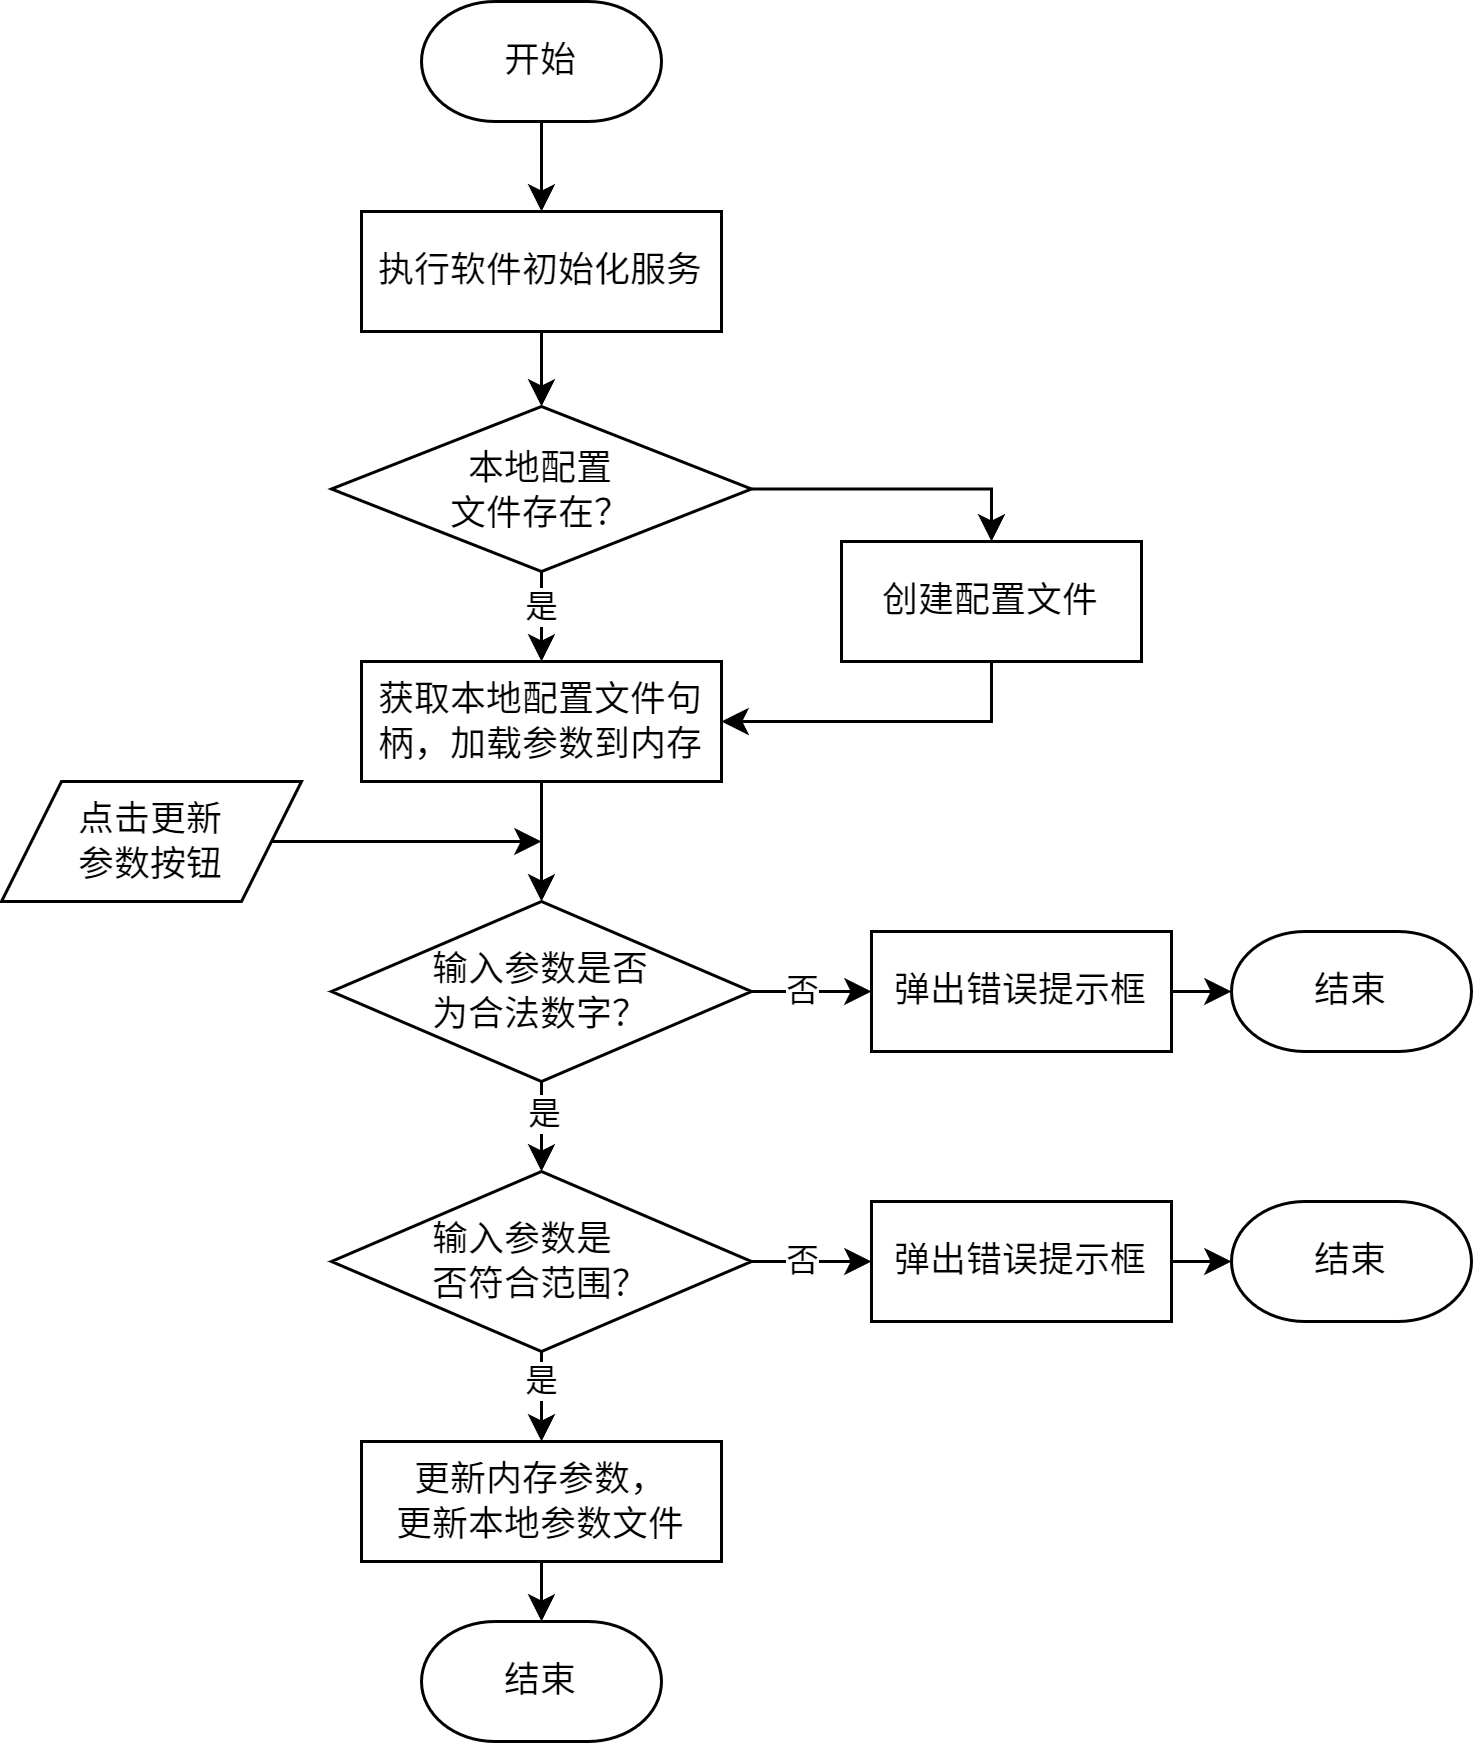
\includegraphics[height=\linewidth]{../figures/2/Fretha业务-参数设置.drawio.png}
  \caption{Fretha 参数设置模块业务流程}
  \label{fig:fretha_param_module_flow}
\end{figure}
参数设置的主要业务流程如图 \ref{fig:fretha_param_module_flow} 所示,遵循如下原则:(1)所有参数一同更新,避免因参数不匹配导致的数据处理错误;(2)每个参数需要在其有意义的范围内,避免无意义的值。
FRET成像参数是一批参数,参数间存在依赖关系,比如测定参数$G$、$k$、$\varepsilon_{A}/\varepsilon_{D}$时需要计算敏化发射荧光$F_C$,根据公式 \ref{eq:fc} 所示,$F_C$的确定与$a$、$b$、$c$、$d$密切相关,因此依赖参数$a$、$b$、$c$、$d$。
强制所有参数一同更新可以避免用户单独设置某一参数而导致参数之间不匹配等问题。
因此,在点击“更新参数”按钮时,若无法从界面中的每个参数输入框都解析到合法的数字,那么本次更新参数就会失败。

FRET成像参数一般比较稳定,一般2到3个月才需要重新测量,因此需要持久化到本地,以供多次处理数据时使用。
Fretha的本地参数文件保存为可执行程序同级目录下的“config.ini”中。在软件初始化阶段,会自动检测并应用本地配置文件中的参数。
用户可通过保存多套配置文件,在使用时替换目标配置文件,快速进行参数配置的切换。

\subsection{数据检验模块}
\label{sec:数据检验模块}

FRET双杂交分析需要处理一批FRET图像文件,因此需要对输入数据的完备性进行检验识别。
该模块的作用有以下两个方面:一方面通过模式识别FRET合法数据,避免了异常输入导致的运行错误;
另一方面,在这一模块会将FRET批数据的视野子文件夹进行解析和类型识别,为后续数据处理提供对子文件夹的不同操作。

基于图 \ref{fig:fretscope_data_struct} 所示数据结构,数据检验业务的流程如图 \ref{fig:fretha_data_check_flow} 所示。
其中,检查子文件夹类型是通过图 \ref{fig:fretscope_data_struct} 进行匹配的,当且仅当子文件夹中同时存在“DA.tif”、“DD.tif”和“AA.tif”图片文件时,当前子文件夹会被识别为FRET视野,并在视野表格模型中记录。
其他情况的子文件夹会被记作“Unknown”文件夹,在后续FRET图像处理或者自动处理中被跳过。
这种检查还会对图像数据是否可读进行检查。
\begin{figure}[htbp]
    \centering
    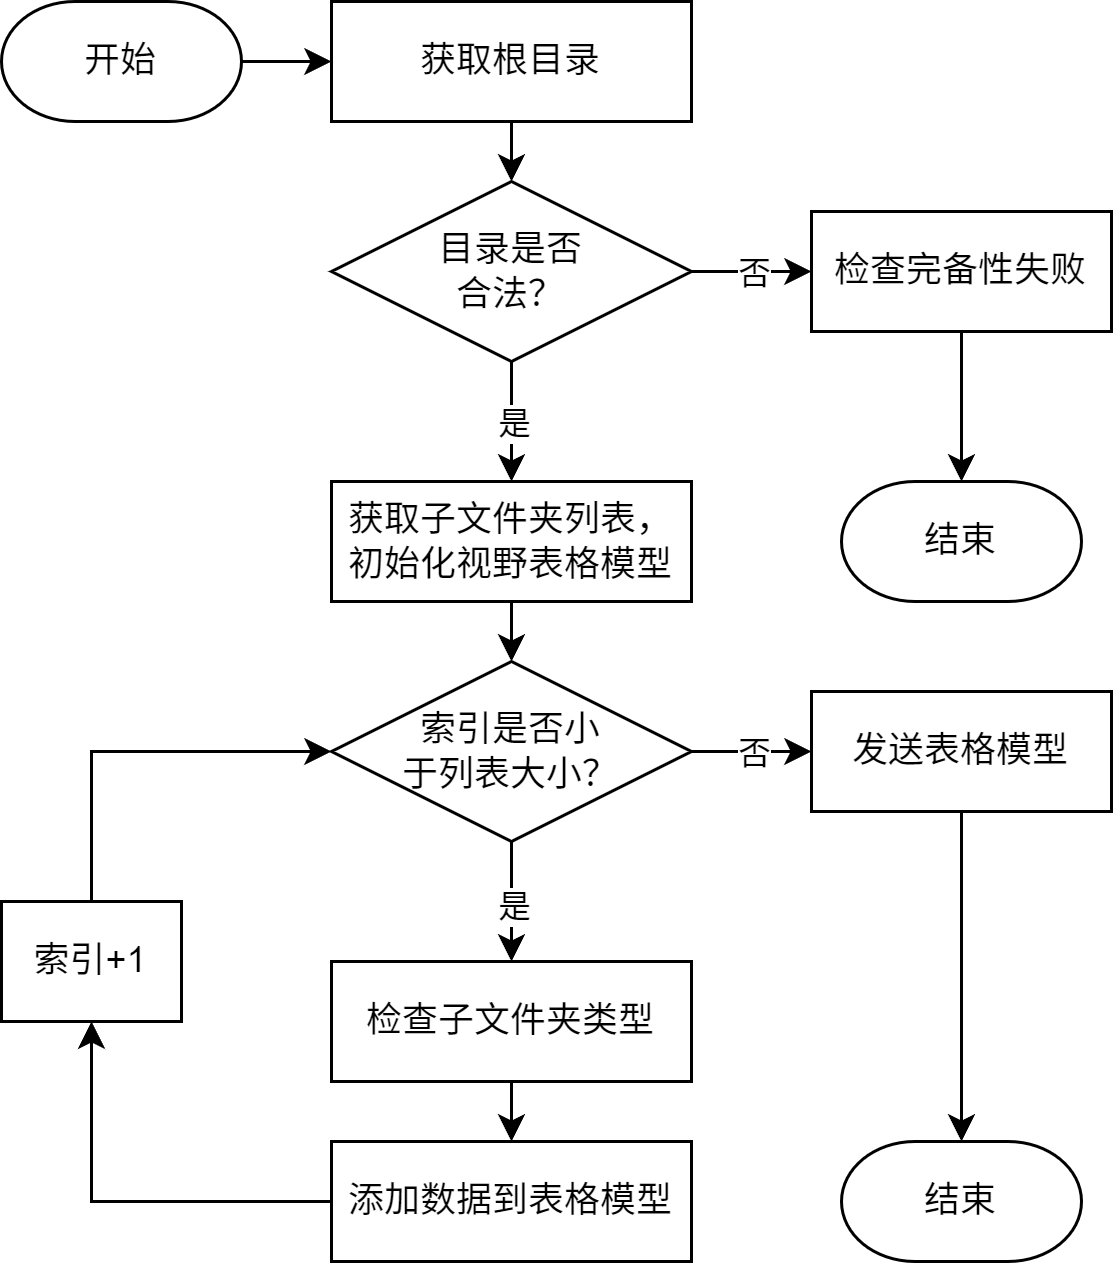
\includegraphics[width=0.65\linewidth]{../figures/2/Fretha业务-数据检验.drawio.png}
    \caption{Fretha数据检验业务主流程图}
    \label{fig:fretha_data_check_flow}
\end{figure}

\subsection{FRET图像处理模块}
\label{sec:FRET图像处理模块}
FRET图像处理模块是对FRET三通道图像进行ROI标注等图像处理分析的模块,其界面主要分为ROI绘制区和状态栏区,如图 \ref{fig:fretha_imageprocess_ui} 所示。
\begin{figure}[htbp]
    \centering
    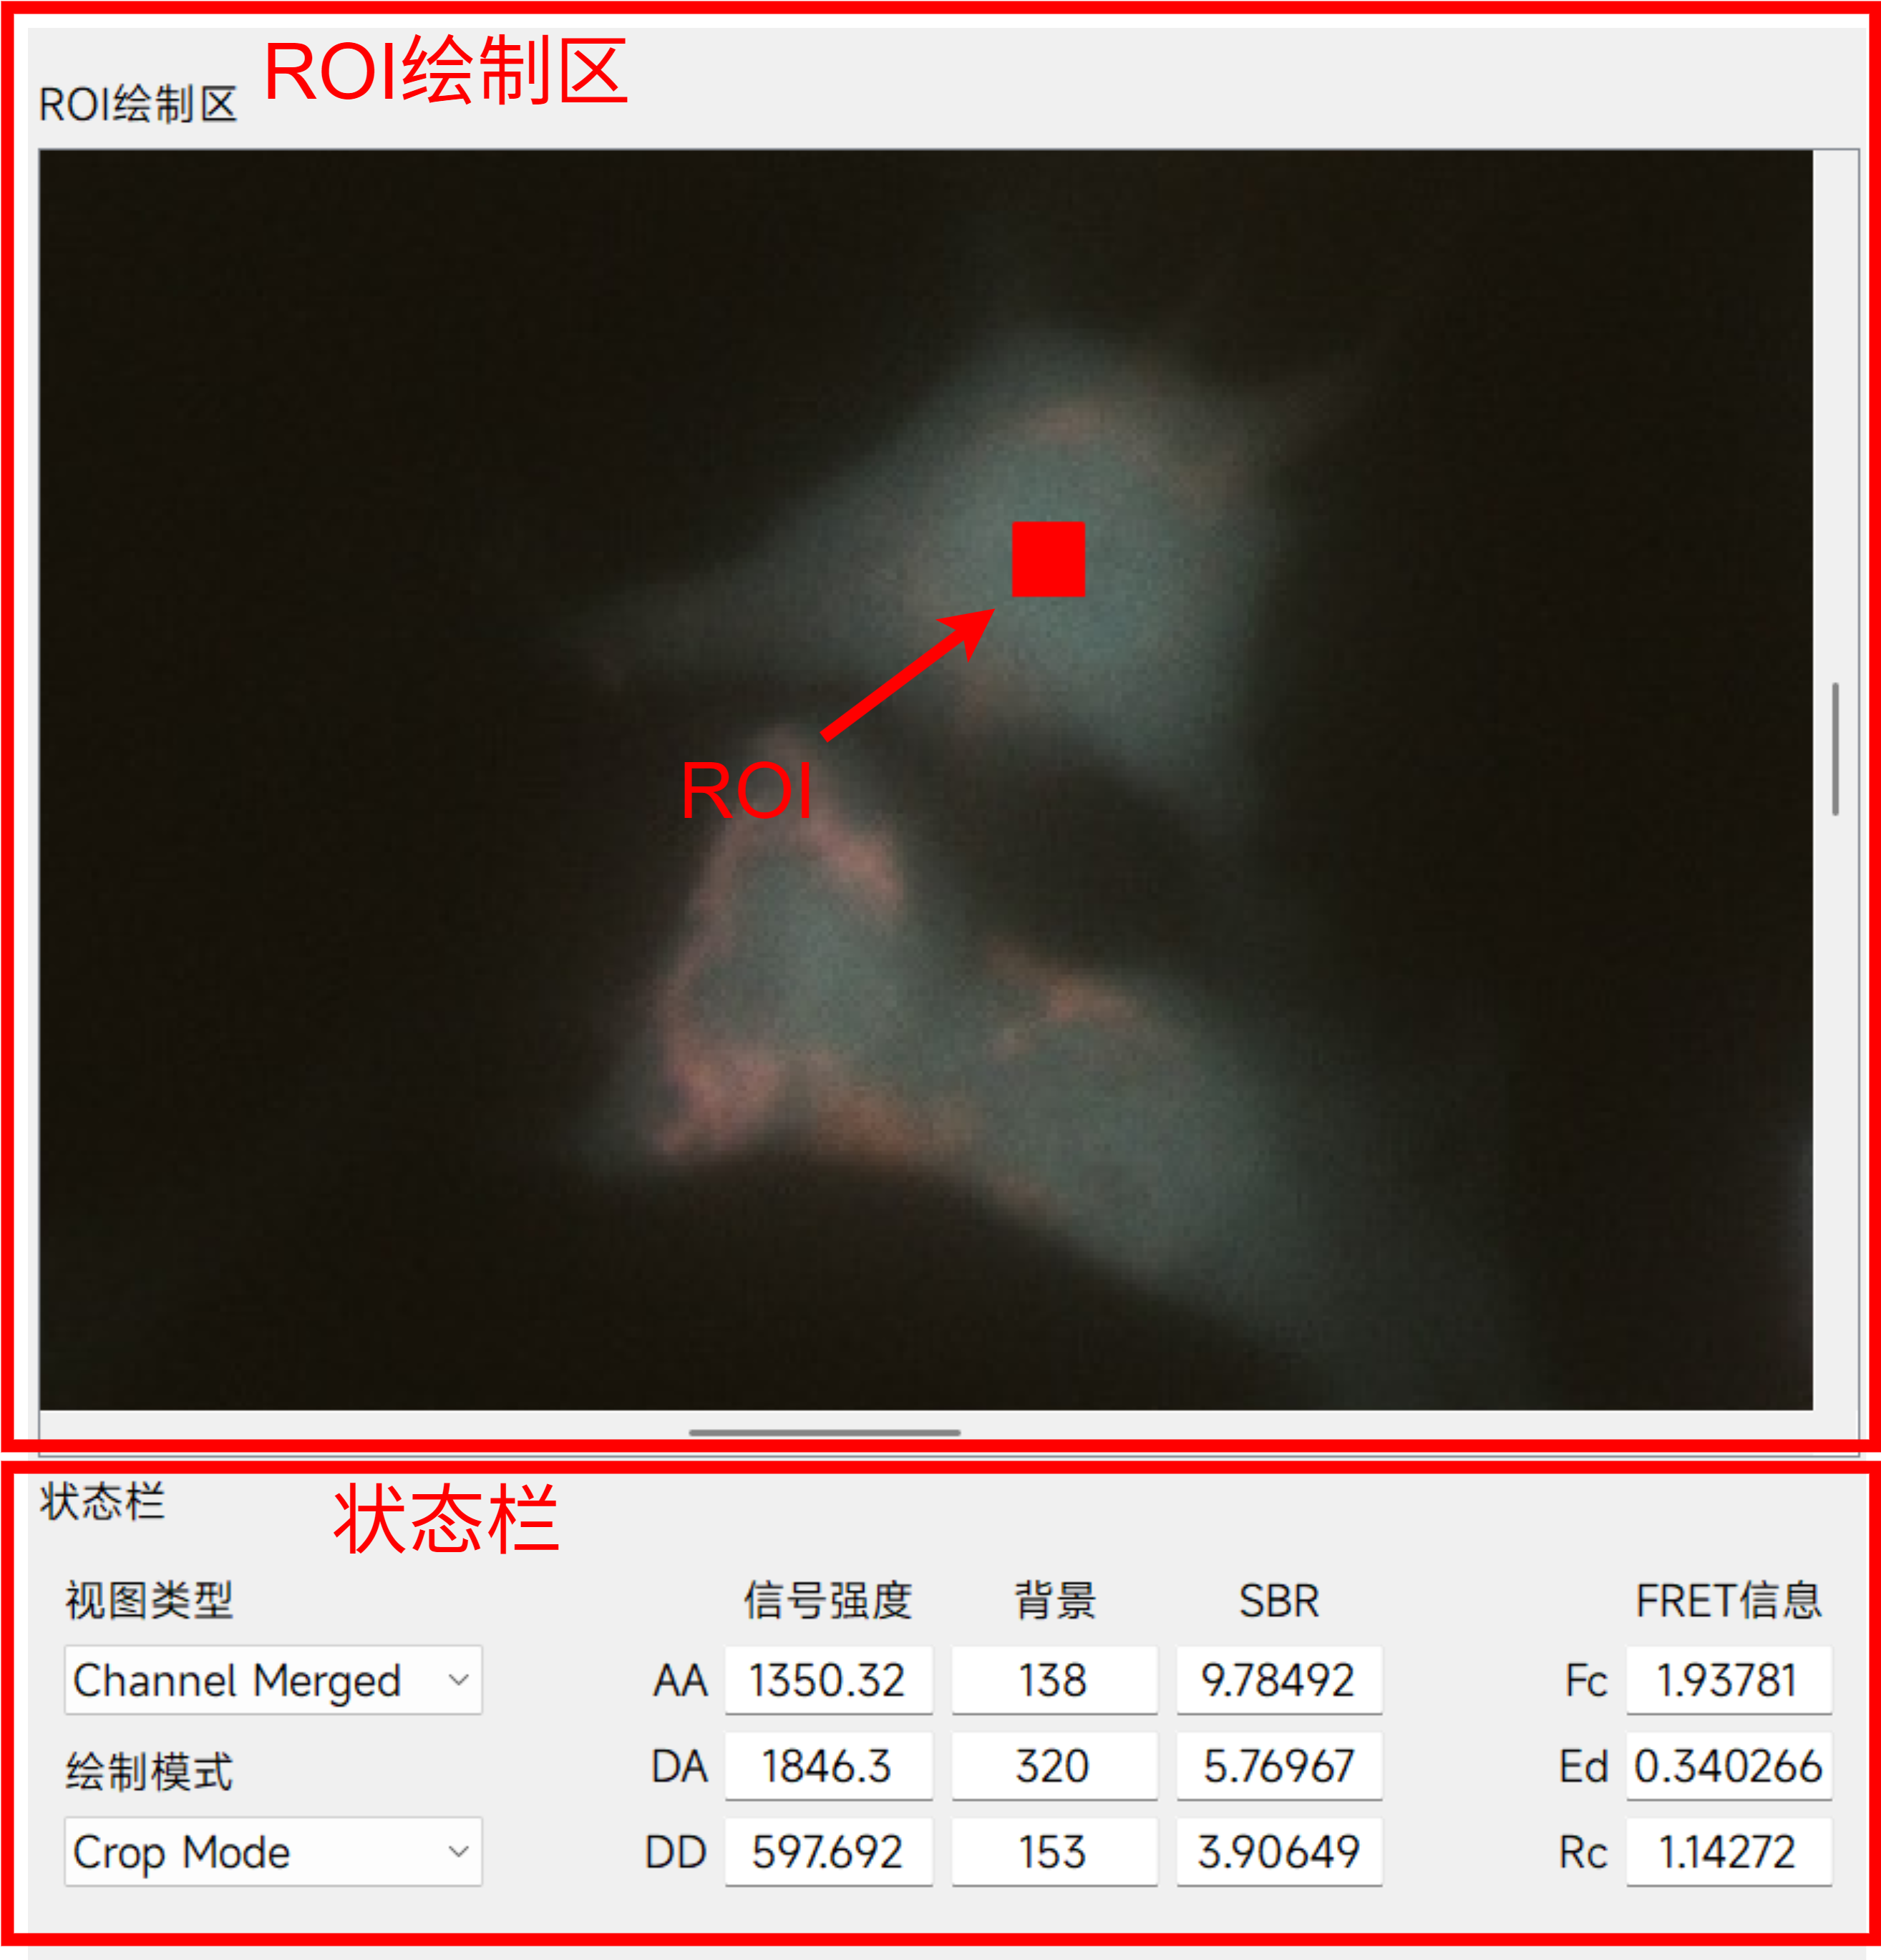
\includegraphics[width=0.6\linewidth]{../figures/2/Fretha图像处理界面.drawio.png}
    \caption{Fretha图像处理模块界面}
    \label{fig:fretha_imageprocess_ui}
\end{figure}
在FRET图像处理工作里,手动选取感兴趣区域ROI是一个基础且关键的操作,它能帮助分析人员聚焦于特定区域,进行更精确的数据处理与分析。
为实现图像处理过程中 ROI 的手动选取功能,Fretha 借助 Qt 框架提供的 QGraphicsView 类,开发了自定义的 FretGraphicsView 类。
QGraphicsView 是 Qt 用于可视化和交互处理二维图形场景的重要类,具备丰富的功能和良好的可扩展性,为 FretGraphicsView 的实现提供了有力支撑。

FretGraphicsView 类中设计了一个基于QRectItem的ROI 成员,它能够在视图中直观呈现 ROI 的大小和位置,方便用户确认所选区域。
设定ROI的绘制模式为“Crop Mode”截取模式时,此时会根据鼠标和ROI边框的位置决定鼠标的编辑功能,包括ROI的创建、移动、缩放等操作。
切换绘制模式为“Stamp”邮戳模式,ROI的大小将会被固定,从而快速圈选多个大小一致的ROI。

Fretha的状态栏中提供了视图类型切换选项,在数据处理中可以辅助圈点,支持的视图类型如表 \ref{tab:fretha_viewtype_list} 所示。
\begin{table}[htbp]
  \centering
  \caption[FRET图像视图类型]{FRET图像视图类型}
  \label{tab:fretha_viewtype_list}
    \begin{tabular}{cc}
      \toprule[1.5pt]
      {视图名} & {说明} \\
      \midrule
      Channel Merged & 三通道归一合成图 \\
      DD Normalized & DD通道的归一化增强图 \\
      DA Normalized & DA通道的归一化增强图 \\
      AA Normalized & AA通道的归一化增强图 \\
      $R_C$ Pseudo & $R_C$逐像素数值伪彩图 \\
      $E_D$ Pseudo & $E_D$逐像素数值伪彩图 \\
      \bottomrule[1.5pt]
    \end{tabular}
\end{table}
归一化增强图包括DD、DA、AA通道分别归一化的增强视图以及三通道归一化合成图。
由于FRET成像系统的相机的量程为$[0,65535]$,计算机显示渲染机制里显示会将65535的灰度值设为白色,而0的灰度值设为黑色,这样会导致图像的对比度低而不利于观察。
通过表 \ref{tab:算法接口} 中的 minMaxNormalization 算法,可以对图像进行全局线性归一化,从而增强图像的对比度。
三通道归一化合并图则是将三个通道的归一化增强图分别作为RGB色彩通道合并成一幅彩色图像,以便于用户直观地观察三通道的信号分布,无需切换通道。
通过FretImageProcessor进行逐像素FRET计算得到$E_D$和$R_C$逐像素矩阵,然后归一化后赋予伪彩,得到用于显示FRET信息的逐像素伪彩图。
\begin{table}[htbp]
  \centering
  \caption[FRET圈点状态栏显示内容]{FRET圈点状态栏显示内容}
  \label{tab:fret_statusbar_list}
      \begin{tabular}{cc}
      \toprule[1.5pt]
      {信息} & {说明} \\
      \midrule
      DD通道信号 & DD通道的ROI内灰度均值 \\
      DA通道信号 & DA通道的ROI内灰度均值 \\
      AA通道信号 & AA通道的ROI内灰度均值 \\
      DD通道背景 & DD通道的视野背景灰度值 \\
      DA通道背景 & DA通道的视野背景灰度值 \\
      AA通道背景 & AA通道的视野背景灰度值 \\
      DD通道SBR & DD通道的信号背景比 \\
      DA通道SBR & DA通道的信号背景比 \\
      AA通道SBR & AA通道的信号背景比 \\
      $F_C$ & 敏化发射的荧光强度 \\
      $E_D$ & 供体视角的表观FRET效率 \\
      $R_C$ & 受体与供体的浓度比 \\
      \bottomrule[1.5pt]
    \end{tabular}
\end{table}

Fretha状态栏能够清晰展示当前视野及ROI的状态信息,如当前视野的三通道背景灰度值、ROI信号的三通道信号背景比(Signal-Background Ratio, SBR)等,还可以显示使用当前ROI提供的扣除背景灰度值后的$I_{DD}$、$I_{DA}$和$I_{DD}$,其中所有显示内容如表 \ref{tab:fret_statusbar_list} 所示。
FretGraphicsView 通过自定义鼠标释放事件的信号,实现了与数据访问层的数据交互。
当用户完成 ROI 选取并释放鼠标时,FretGraphicsView 会将 ROI 的坐标和大小信息传递给数据访问层。
数据访问层依据当前视野索引,从数据模型中读取相应的三通道图像文件,并且从ROI信息提取FRET信号。
在获得了$I_{DD}$、$I_{DA}$和$I_{DD}$后,Fretha后台会自动扣除每个通道的背景灰度,然后根据公式 \ref{eq:fc},调用后台的FretCalculator计算出敏化发射的荧光强度$F_C$、$E_D$,$R_C$,并显示在状态栏中,方便用户获取处理结果,为ROI的保留和移除提供判断依据。
这种基于 QGraphicsView 扩展的设计,有效提升了 ROI 选取的灵活性和准确性。 

\subsection{数据管理模块}
\label{sec:数据管理模块}

数据管理模块支持对数据的实时操作,可以对于图像处理模块获得的数据,进行异常数据筛选、数据追踪、数据导入、数据导出、计算入口等数据管理控制功能。

一条数据类型FretDataPiece中包含数据如表 \ref{tab:数据项内容定义} 所示。
可以看出,FretDataPiece包含了一个ROI对应的所有原始信息,如ROI的位置、大小、信号强度、视野等;
同时,还包含了计算后的$E_D$、$E_A$、$R_C$、$1/R_C$等中间参数,可以直接被用于后续的数据处理。

\begin{table}[htbp]
  \centering
  \caption{FretDataPiece数据类型}
  \label{tab:数据项内容定义}
    \begin{tabular}{cc}
      \toprule[1.5pt]
      {信息} & {说明} \\
      \midrule
      $I_{DD}$ & ROI在DD通道扣除背景后的信号强度 \\
      $I_{DA}$ & ROI在DA通道扣除背景后的信号强度 \\
      $I_{AA}$ & ROI在DD通道扣除背景后的信号强度 \\
      $E_D$ & 根据$I_{DD}$、$I_{DA}$、$I_{AA}$计算的$E_D$ \\
      $R_C$ & 根据$I_{DD}$、$I_{DA}$、$I_{AA}$计算的$R_C$ \\
      $E_A$ & 根据$I_{DD}$、$I_{DA}$、$I_{AA}$计算的$E_A$ \\
      $1/R_C$ & $R_C$的倒数 \\
      $A_{est}$ & 供体分子数的估计值 \\
      $D_{est}$ & 受体分子数的估计值 \\
      $x$ & ROI的横坐标 \\
      $y$ & ROI的纵坐标 \\
      $w$ & ROI的宽度 \\
      $h$ & ROI的高度 \\
      $view$ & ROI隶属的视野\\
      \bottomrule[1.5pt]
    \end{tabular}
\end{table}

为保证数据符合实际物理意义,避免中间数据的异常值对后续计算产生影响,数据管理模块提供了数据筛选功能。
点击“筛选数据”,数据管理模块会对数据根据物理定义和统计学准则进行筛选,剔除异常数据。
具体数据筛选流程实施主要包括两个方面:

第一是对$I_{DD}$、$I_{DA}$、$I_{AA}$基于物理约束的初步数据清洗:
针对各数值型变量 \( x_i \),依据其预设的物理合理区间 \( [L_i, U_i] \) 执行有效性校验。构建如下二元判别函数:
\begin{equation}
  \delta(x_i) = 
  \begin{cases} 
    1, & x_i \notin [L_i, U_i]  \\
    0, & x_i \in [L_i, U_i]
  \end{cases} ,
\end{equation}
当 \( \delta(x_i) = 1 \) 时,判定该数据点为物理意义上的异常值并予以剔除。

第二是对中间计算的FRET计算结果$E_D$、$E_A$、$R_C$统计离群点检测:
对经初步清洗后的数据子集 \( E_D \)、\( E_A \)和$R_C$,分别计算变量的样本均值 \( \mu \) 和样本标准差 \( \sigma \),计算公式如下:
\begin{equation}
  \mu = \frac{1}{n}\sum_{i=1}^n x_i, \quad \sigma = \sqrt{\frac{1}{n - 1}\sum_{i=1}^n (x_i - \mu)^2}.
\end{equation}
采用3σ准则设定离群阈值,即构建判别区间 \( [\mu - 3\sigma, \mu + 3\sigma] \)。超出该区间的观测值均判定为统计离群点并剔除。


数据导出用于保存数据处理时的ROI信息。
在完成FRET图像处理和ROI绘制选取后,需要保存ROI的结果,以便后续分析或者修改编辑。
在数据管理模块点击“导出数据”按钮,Fretha将会导出数据区记录的所有数据,每一条数据都会按照FretDataPiece定义进行逐列导出,文件格式为CSV文件。
数据导入功能则可以读取Fretha导出的CSV文件,然后解析其中的数据按照FretDataPiece的格式。

数据管理区的操作为:点击“添加数据”按钮或者使用快捷键“A”,可以添加当前状态栏中的数据到数据表格中;
点击“删除数据”按钮或者使用快捷键“D”,可以删除数据表格中选中的数据;
点击“清空数据”按钮或者使用快捷键“C”,可以清空数据表格中的所有数据;
点击“开始计算”按钮,软件将调用FretTwoHybridSolver等算法对数据表格中的数据进行FRET双杂交分析求解计算,并将结果显示在结果可视化模块中,然后切换软件界面到结果可视化模块。
此外,基于Qt提供的信号与槽机制,还支持了数据的反向追溯功能,即在数据表格中点击某一条数据,软件会根据这条数据的位置和形状信息,在图像显示上显示该条数据对应的ROI位置,以方便检查数据处理中标注错误的ROI。
将数据中的数据模型被点击的事件信号与 FretGraphicsView 控件中的回调槽函数绑定后,FretGraphicView 模型可以接收到来自所选数据的信息,按照所选数据项中ROI的$x$、$y$、$w$和$h$绘制ROI到FretGraphicsView控件上,并将FretGraphicsView的视角中心移动到所选数据的ROI中心,以便用户更加直观地查看数据的位置和形状。

\subsection{结果可视化模块}
\label{sec:结果可视化模块}
FRET双杂交分析的输出结果包含双杂交计算的参数结果与拟合曲线图。
其中,$E_{A,max}$、$E_{D,max}$、$n_D/n_A$、$K_{d,EFF}$等参数以数据框形式展示;
拟合曲线图通过将双杂交理论拟合曲线与实验散点数据同图可视化,实现对拟合效果的直观评估,进而验证FRET双杂交分析结果的可靠性。

结果可视化模块的界面组成如图 \ref{fig:Fretha结果可视化模块界面} 所示,主要包含以下三个功能区域:
(1)视图选择:切换FRET双杂交分析算法,更新对应的结果视图;
(2)图表分析:显示FRET双杂交分析的拟合趋势线和散点图;
(3)操作按钮:结果保存按钮和返回圈点界面按钮。

点击视图按钮可以切换不同FRET双杂交分析的算法方法的计算结果,更新图表分析区域显示的方法。
在可视化结果展示区域,软件将拟合结果与实验数据同步呈现在同一坐标系中,便于用户进行直接比对。
拟合曲线是基于拟合参数计算得到的理论数据点连接而成的平滑曲线,实验数据则以离散点形式展示,用户可以直观检查拟合计算的效果和误差大小。
可视化界面基于QChart组件作图绘制,根据一批数据(FretDataRecord)的数据范围分布,自动优化坐标轴刻度范围,以提升数据可视化的清晰度。

在 L-FRET 视图模式下,软件集成了数据预处理 BIN 功能,允许用户通过合并供体 - 受体浓度在相同区间的数据进行预处理数据\upcite{供体-受体浓度比}。如图 \ref{fig:Fretha结果可视化模块界面},通过设置界面中数据合并预处理的参数,然后点击“更新”按钮即可应用数据预处理,在L-FRET拟合效果不理想时可以用来优化数据处理结果。
\begin{figure}[htbp]
  \centering
  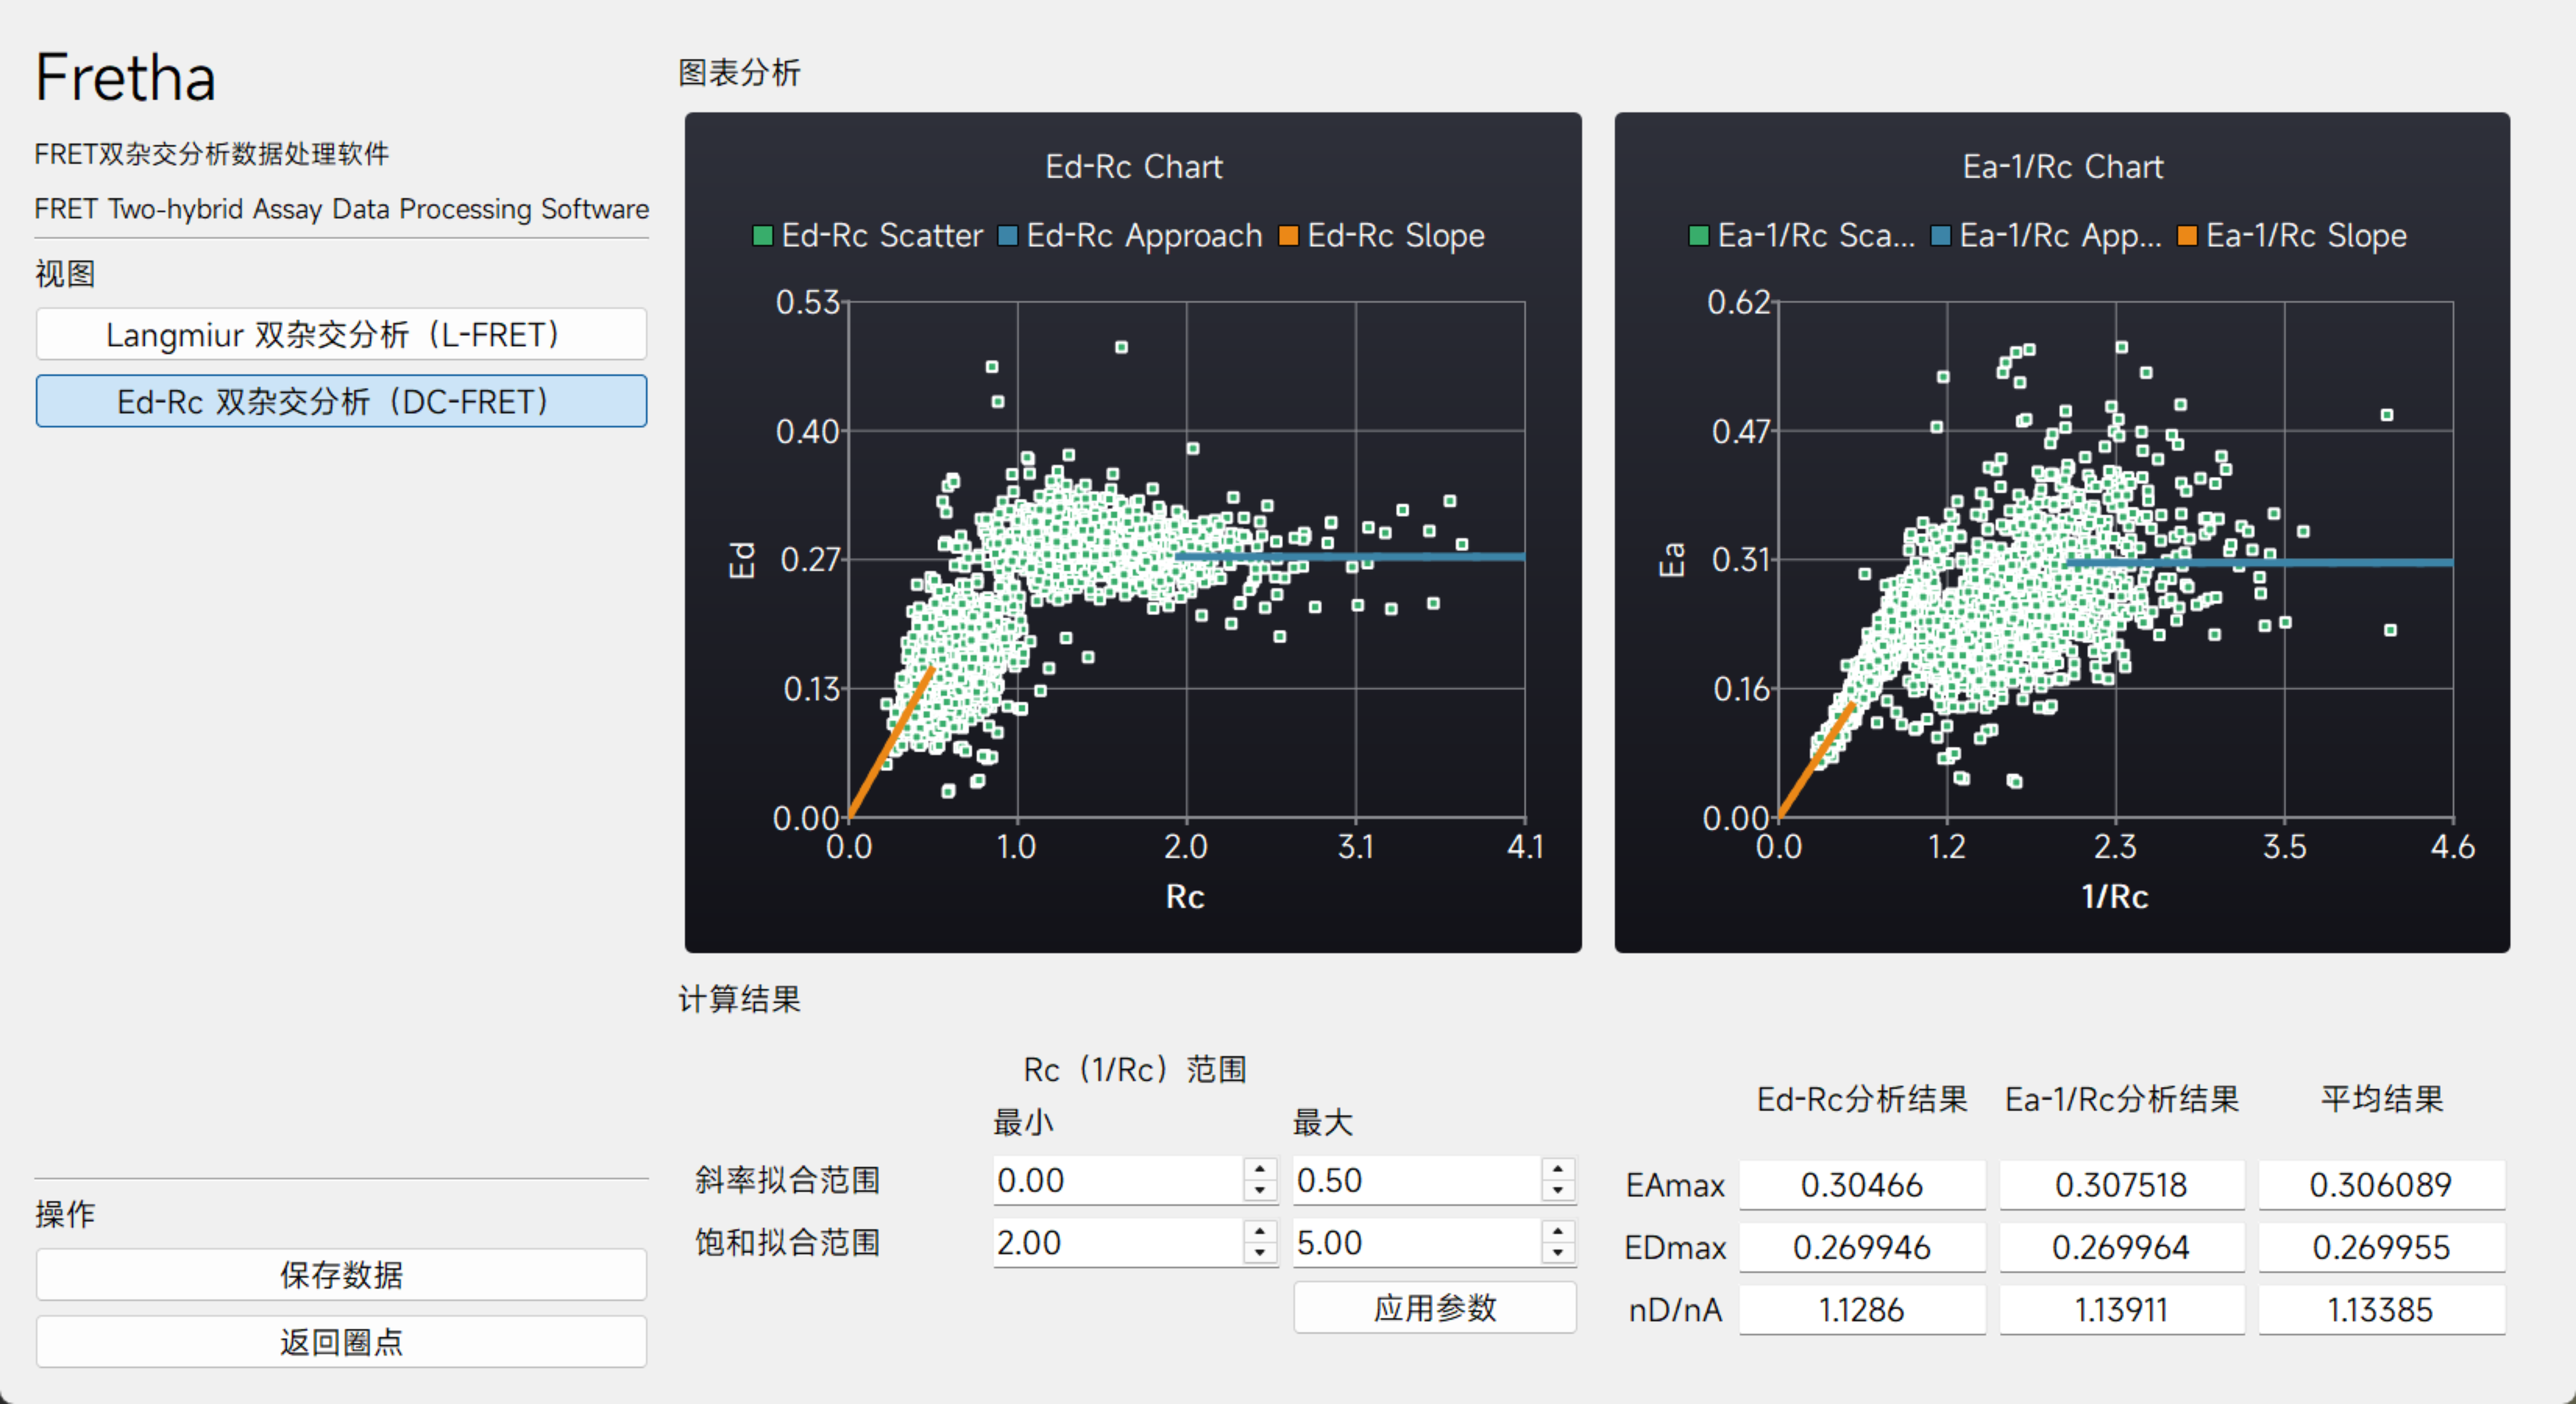
\includegraphics[width=0.9\linewidth]{../figures/2/DC-FRET结果界面.drawio.png}
  \caption{Fretha DC-FRET视图}
  \label{fig:fretha_dc_fret}
\end{figure}

DC-FRET视图的界面如图 \ref{fig:fretha_dc_fret} 所示。
在DC-FRET视图模式下,软件能显示出DC-FRET的拟合结果,包括$E_{A,max}$、$E_{D,max}$、$n_D/n_A$,以及拟合曲线和实验数据的对比图。
界面中设计了调整线性拟合参数的设置栏,用户可以调整$R_C$($1/R_C$)的数据范围,点击“更新”按钮以应用范围参数,用来处理复杂的数据。

点击“保存结果”按钮后,系统将同步存储拟合结果数据、可视化图像及实验数据,保存结果如图表所示。
\begin{table}[htbp]
  \centering
  \caption{结果保存生成文件}
  \label{tab:fretha_result_list}
    \begin{tabular}{cc}
      \toprule[1.5pt]
      {文件名} & {说明} \\
      \midrule
      Ea-Rda图.png & $E_A$-$1/R_C$散点和趋势线图 \\
      Ed-Rad图.png & $E_D$-$R_C$散点和趋势线图 \\
      Ea-Dfree图.png & $E_A$-$D_{free}$散点和趋势线图 \\
      Ed-Afree图.png & $E_D$-$A_{free}$散点和趋势线图 \\
      FretThaData.csv & FRET双杂交分析结果数据 \\
      FretThaResults.csv & FRET双杂交分析结果拟合参数 \\
      \bottomrule[1.5pt]
    \end{tabular}
\end{table}
其中,实验数据与拟合参数的原始数值将以 CSV 文件格式进行保存,该文件包含可直接用于其他科研绘图软件的数据记录,从而支持用户在不同的可视化工具中进行科研绘图与再处理。
这一功能设计保障了实验结果的完整留存,为科研工作者提供了灵活的数据导出与再分析解决方案。

\section{本章小结}
本章系统阐述了 FRET 双杂交分析数据处理软件 Fretha 的设计和实现。
首先,本章分析了FRETScope成像系统的数据特点和FRET双杂交分析数据处理流程。
基于上述需求分析,Fretha在模块上划分成了成像参数设置、数据检验、FRET图像处理、数据管理和结果可视化五个主要功能模块。
其次,Fretha采用了表现层、业务层、数据访问层和数据层的四层架构体系,从而实现了软件的解耦设计。
基于OpenCV和Dlib等开源计算库,本章构建了包含 FRET 定量计算器、图像处理器和双杂交求解器的后台接口,实现了 E-FRET、 $3^3$-FRET、DC-FRET、L-FRET等多模态FRET算法。
最后,本文基于Qt框架和C++编程语言完成了各个模块的界面实现和业务编写,实现了Fretha软件的开发实现。
基于Fretha的分层架构设计,软件各个模块之间的耦合度较低,数据在Fretha内部实现了统一管理和传输。
Fretha是一款拥有用户友好界面的专业数据处理软件,实现了从原始数据到化学计量比结果的标准化数据流程,有效提高了FRET双杂交分析技术的简单化、规范化程度。